% ManuVox, IEEE conference version (IEEEtran). The full version, with the appendices, is
% ../main.tex; this version cites it as the extended version. Build: see ../README.md
% (cd paper/ieee; tectonic main_ieee.tex).
% Every number in the text is a macro \V{key} from ../tables/numbers.tex, written by
% scripts/paper_tables.py from the result files; the tables in tables/ come from the same
% generator (title above, full caption as a note below). Do not type numbers by hand.
% The abstract, introduction, conclusion and acknowledgment are shared with the full version
% (../sections/); the other sections are condensed versions in sections/.
\documentclass[conference]{IEEEtran}
\usepackage[T1]{fontenc}
\usepackage{cite}
\usepackage{amsmath}
\usepackage{graphicx}
\usepackage{booktabs}
\usepackage{array}
\usepackage{multirow}
\usepackage{makecell}
\usepackage{xcolor}
\usepackage{tikz}
\usetikzlibrary{arrows.meta,positioning,fit,calc}
\usepackage{microtype}
\usepackage[hidelinks]{hyperref}
% PDF metadata: title and author only.
\hypersetup{pdftitle={ManuVox: Auditing the Train\textendash Serve Gap of a Landmark-Based Sign
  Recognizer on a Laptop}, pdfauthor={Swapnil Shukla}, pdfcreator={}, pdfproducer={}}

% ---------------------------------------------------------------- numbers
\makeatletter
\newcommand{\V}[1]{\ifcsname v@#1\endcsname\csname v@#1\endcsname\else
  \PackageError{numbers}{Undefined number key #1 (rerun scripts/paper_tables.py)}{}\textbf{??#1??}\fi}
\makeatother
% Generated by scripts/paper_tables.py -- do not edit by hand.
% Each number quoted in the paper is \V{key}; sources: paper/data/macro_sources.json.
\expandafter\newcommand\csname v@asp.train\endcsname{0.723}
\expandafter\newcommand\csname v@b.chrome\endcsname{157}
\expandafter\newcommand\csname v@b.wasm1.p50\endcsname{18.6}
\expandafter\newcommand\csname v@b.wasm1.p95\endcsname{26.1}
\expandafter\newcommand\csname v@b.wasm2.p50\endcsname{29.9}
\expandafter\newcommand\csname v@b.wasm2.p95\endcsname{41.5}
\expandafter\newcommand\csname v@b.wasm4.p50\endcsname{32.3}
\expandafter\newcommand\csname v@b.wasm4.p95\endcsname{54.4}
\expandafter\newcommand\csname v@b.webgpu1.p50\endcsname{50.1}
\expandafter\newcommand\csname v@b.webgpu1.p95\endcsname{66.4}
\expandafter\newcommand\csname v@budget.fps\endcsname{15}
\expandafter\newcommand\csname v@budget.ms\endcsname{60}
\expandafter\newcommand\csname v@cal.T\endcsname{0.868}
\expandafter\newcommand\csname v@cal.bins\endcsname{15}
\expandafter\newcommand\csname v@cal.targetprec\endcsname{80}
\expandafter\newcommand\csname v@cal.test.cov\endcsname{72.8}
\expandafter\newcommand\csname v@cal.test.ece0\endcsname{0.083}
\expandafter\newcommand\csname v@cal.test.ece0ci\endcsname{[0.077, 0.089]}
\expandafter\newcommand\csname v@cal.test.ece1\endcsname{0.033}
\expandafter\newcommand\csname v@cal.test.ece1ci\endcsname{[0.029, 0.040]}
\expandafter\newcommand\csname v@cal.test.n\endcsname{16,242}
\expandafter\newcommand\csname v@cal.test.net\endcsname{0.47}
\expandafter\newcommand\csname v@cal.test.nll0\endcsname{1.614}
\expandafter\newcommand\csname v@cal.test.nll1\endcsname{1.557}
\expandafter\newcommand\csname v@cal.test.rejright\endcsname{13}
\expandafter\newcommand\csname v@cal.test.rejwrong\endcsname{58}
\expandafter\newcommand\csname v@cal.test.sel\endcsname{82.0}
\expandafter\newcommand\csname v@cal.test.top1\endcsname{68.4}
\expandafter\newcommand\csname v@cal.test.top3\endcsname{82.3}
\expandafter\newcommand\csname v@cal.thr\endcsname{48.8}
\expandafter\newcommand\csname v@cal.val.cov\endcsname{73.5}
\expandafter\newcommand\csname v@cal.val.ece0\endcsname{0.076}
\expandafter\newcommand\csname v@cal.val.ece1\endcsname{0.045}
\expandafter\newcommand\csname v@cal.val.sel\endcsname{80.8}
\expandafter\newcommand\csname v@cit.all.glosses\endcsname{2,731}
\expandafter\newcommand\csname v@cit.all.signers\endcsname{52}
\expandafter\newcommand\csname v@cit.all.testsigners\endcsname{11}
\expandafter\newcommand\csname v@cit.all.trainsigners\endcsname{35}
\expandafter\newcommand\csname v@cit.all.valsigners\endcsname{6}
\expandafter\newcommand\csname v@cit.all.videos\endcsname{83,399}
\expandafter\newcommand\csname v@cit.excluded\endcsname{13}
\expandafter\newcommand\csname v@cit.map.exact\endcsname{171}
\expandafter\newcommand\csname v@cit.map.mapped\endcsname{236}
\expandafter\newcommand\csname v@cit.map.synonym\endcsname{30}
\expandafter\newcommand\csname v@cit.map.unmapped\endcsname{14}
\expandafter\newcommand\csname v@cit.map.variant\endcsname{35}
\expandafter\newcommand\csname v@cit.map.vocabulary\endcsname{250}
\expandafter\newcommand\csname v@cit.rule.exact\endcsname{2,083}
\expandafter\newcommand\csname v@cit.rule.synonym\endcsname{481}
\expandafter\newcommand\csname v@cit.rule.variant\endcsname{959}
\expandafter\newcommand\csname v@cit.signers\endcsname{11}
\expandafter\newcommand\csname v@cit.signs\endcsname{236}
\expandafter\newcommand\csname v@cit.v2.cov\endcsname{31.1}
\expandafter\newcommand\csname v@cit.v2.drop\endcsname{25.3}
\expandafter\newcommand\csname v@cit.v2.ece\endcsname{0.066}
\expandafter\newcommand\csname v@cit.v2.eceraw\endcsname{0.147}
\expandafter\newcommand\csname v@cit.v2.exact\endcsname{48.6}
\expandafter\newcommand\csname v@cit.v2.sel\endcsname{79.8}
\expandafter\newcommand\csname v@cit.v2.sigmax\endcsname{50.0}
\expandafter\newcommand\csname v@cit.v2.sigmin\endcsname{31.4}
\expandafter\newcommand\csname v@cit.v2.synonym\endcsname{43.9}
\expandafter\newcommand\csname v@cit.v2.top1\endcsname{43.1}
\expandafter\newcommand\csname v@cit.v2.top1ci\endcsname{[41.5, 44.8]}
\expandafter\newcommand\csname v@cit.v2.top1cis\endcsname{[39.3, 46.6]}
\expandafter\newcommand\csname v@cit.v2.top3\endcsname{57.6}
\expandafter\newcommand\csname v@cit.v2.variant\endcsname{30.9}
\expandafter\newcommand\csname v@cit.v3.cov\endcsname{88.1}
\expandafter\newcommand\csname v@cit.v3.ece\endcsname{0.066}
\expandafter\newcommand\csname v@cit.v3.eceraw\endcsname{0.150}
\expandafter\newcommand\csname v@cit.v3.exact\endcsname{91.1}
\expandafter\newcommand\csname v@cit.v3.sel\endcsname{97.3}
\expandafter\newcommand\csname v@cit.v3.sigmax\endcsname{97.5}
\expandafter\newcommand\csname v@cit.v3.sigmin\endcsname{87.1}
\expandafter\newcommand\csname v@cit.v3.synonym\endcsname{93.6}
\expandafter\newcommand\csname v@cit.v3.top1\endcsname{92.1}
\expandafter\newcommand\csname v@cit.v3.top1ci\endcsname{[91.2, 93.0]}
\expandafter\newcommand\csname v@cit.v3.top1cis\endcsname{[90.3, 93.9]}
\expandafter\newcommand\csname v@cit.v3.top3\endcsname{97.2}
\expandafter\newcommand\csname v@cit.v3.variant\endcsname{93.6}
\expandafter\newcommand\csname v@cit.videos\endcsname{3,523}
\expandafter\newcommand\csname v@cmp.arch.ci\endcsname{[4.5, 5.3]}
\expandafter\newcommand\csname v@cmp.arch.diff\endcsname{+4.9}
\expandafter\newcommand\csname v@cmp.arch.nsigners\endcsname{4}
\expandafter\newcommand\csname v@cmp.arch.p\endcsname{$<$0.001}
\expandafter\newcommand\csname v@cmp.arch.sig\endcsname{significant}
\expandafter\newcommand\csname v@cmp.arch.signers\endcsname{4}
\expandafter\newcommand\csname v@cmp.family\endcsname{6}
\expandafter\newcommand\csname v@cmp.feat.ci\endcsname{[$-$0.2, 0.6]}
\expandafter\newcommand\csname v@cmp.feat.diff\endcsname{+0.2}
\expandafter\newcommand\csname v@cmp.feat.nsigners\endcsname{4}
\expandafter\newcommand\csname v@cmp.feat.p\endcsname{0.688}
\expandafter\newcommand\csname v@cmp.feat.sig\endcsname{not significant}
\expandafter\newcommand\csname v@cmp.feat.signers\endcsname{1}
\expandafter\newcommand\csname v@cmp.gru.ci\endcsname{[$-$1.9, $-$1.1]}
\expandafter\newcommand\csname v@cmp.gru.diff\endcsname{$-$1.5}
\expandafter\newcommand\csname v@cmp.gru.nsigners\endcsname{4}
\expandafter\newcommand\csname v@cmp.gru.p\endcsname{$<$0.001}
\expandafter\newcommand\csname v@cmp.gru.sig\endcsname{significant}
\expandafter\newcommand\csname v@cmp.gru.signers\endcsname{0}
\expandafter\newcommand\csname v@cmp.n\endcsname{16,242}
\expandafter\newcommand\csname v@cmp.recipe.ci\endcsname{[0.6, 1.4]}
\expandafter\newcommand\csname v@cmp.recipe.diff\endcsname{+1.0}
\expandafter\newcommand\csname v@cmp.recipe.nsigners\endcsname{4}
\expandafter\newcommand\csname v@cmp.recipe.p\endcsname{$<$0.001}
\expandafter\newcommand\csname v@cmp.recipe.sig\endcsname{significant}
\expandafter\newcommand\csname v@cmp.recipe.signers\endcsname{4}
\expandafter\newcommand\csname v@cmp.ship.ci\endcsname{[5.6, 6.5]}
\expandafter\newcommand\csname v@cmp.ship.diff\endcsname{+6.1}
\expandafter\newcommand\csname v@cmp.ship.nsigners\endcsname{4}
\expandafter\newcommand\csname v@cmp.ship.p\endcsname{$<$0.001}
\expandafter\newcommand\csname v@cmp.ship.sig\endcsname{significant}
\expandafter\newcommand\csname v@cmp.ship.signers\endcsname{4}
\expandafter\newcommand\csname v@cmp.tf.ci\endcsname{[$-$0.3, 0.5]}
\expandafter\newcommand\csname v@cmp.tf.diff\endcsname{+0.1}
\expandafter\newcommand\csname v@cmp.tf.nsigners\endcsname{4}
\expandafter\newcommand\csname v@cmp.tf.p\endcsname{0.717}
\expandafter\newcommand\csname v@cmp.tf.sig\endcsname{not significant}
\expandafter\newcommand\csname v@cmp.tf.signers\endcsname{2}
\expandafter\newcommand\csname v@data.excluded\endcsname{6,945}
\expandafter\newcommand\csname v@data.facedist\endcsname{24}
\expandafter\newcommand\csname v@data.frames\endcsname{32}
\expandafter\newcommand\csname v@data.kept\endcsname{87,532}
\expandafter\newcommand\csname v@data.lmface\endcsname{468}
\expandafter\newcommand\csname v@data.lmhand\endcsname{21}
\expandafter\newcommand\csname v@data.lmpose\endcsname{33}
\expandafter\newcommand\csname v@data.lmtotal\endcsname{543}
\expandafter\newcommand\csname v@data.minhand\endcsname{3}
\expandafter\newcommand\csname v@data.mirroredpct\endcsname{43.2}
\expandafter\newcommand\csname v@data.pairdist\endcsname{210}
\expandafter\newcommand\csname v@data.signers\endcsname{21}
\expandafter\newcommand\csname v@data.signmax\endcsname{402}
\expandafter\newcommand\csname v@data.signmin\endcsname{235}
\expandafter\newcommand\csname v@data.signs\endcsname{250}
\expandafter\newcommand\csname v@data.testseq\endcsname{16,242}
\expandafter\newcommand\csname v@data.testsigners\endcsname{4}
\expandafter\newcommand\csname v@data.total\endcsname{94,477}
\expandafter\newcommand\csname v@data.trainseq\endcsname{58,717}
\expandafter\newcommand\csname v@data.trainsigners\endcsname{14}
\expandafter\newcommand\csname v@data.v1points\endcsname{49}
\expandafter\newcommand\csname v@data.v1pose\endcsname{7}
\expandafter\newcommand\csname v@data.v2feat\endcsname{588}
\expandafter\newcommand\csname v@data.v2points\endcsname{59}
\expandafter\newcommand\csname v@data.v2pose\endcsname{17}
\expandafter\newcommand\csname v@data.valseq\endcsname{12,573}
\expandafter\newcommand\csname v@data.valsigners\endcsname{3}
\expandafter\newcommand\csname v@hp.seeds\endcsname{3}
\expandafter\newcommand\csname v@hp.v1.epochs\endcsname{60}
\expandafter\newcommand\csname v@hp.v2.ema\endcsname{0.999}
\expandafter\newcommand\csname v@hp.v2.epochs\endcsname{150}
\expandafter\newcommand\csname v@hw.cores\endcsname{2}
\expandafter\newcommand\csname v@hw.ramgib\endcsname{19.7}
\expandafter\newcommand\csname v@hw.threads\endcsname{4}
\expandafter\newcommand\csname v@lat.p95hi\endcsname{33.9}
\expandafter\newcommand\csname v@lat.p95lo\endcsname{20.7}
\expandafter\newcommand\csname v@lat.v2.p50\endcsname{14.3}
\expandafter\newcommand\csname v@lat.v2.p95\endcsname{21.2}
\expandafter\newcommand\csname v@lat.v3.mb\endcsname{6.9}
\expandafter\newcommand\csname v@lat.v3.p50\endcsname{13.3}
\expandafter\newcommand\csname v@lat.v3.p95\endcsname{31.3}
\expandafter\newcommand\csname v@lg.browserrecords\endcsname{2,250}
\expandafter\newcommand\csname v@lg.cal.py.cov\endcsname{49}
\expandafter\newcommand\csname v@lg.cal.py.ece\endcsname{0.136}
\expandafter\newcommand\csname v@lg.cal.py.net\endcsname{0.16}
\expandafter\newcommand\csname v@lg.cal.py.rejright\endcsname{24}
\expandafter\newcommand\csname v@lg.cal.py.rejwrong\endcsname{70}
\expandafter\newcommand\csname v@lg.cal.py.sel\endcsname{66}
\expandafter\newcommand\csname v@lg.cal.py.xpresence.cov\endcsname{46}
\expandafter\newcommand\csname v@lg.cal.py.xpresence.ece\endcsname{0.176}
\expandafter\newcommand\csname v@lg.cal.py.xpresence.net\endcsname{0.15}
\expandafter\newcommand\csname v@lg.cal.py.xpresence.rejright\endcsname{33}
\expandafter\newcommand\csname v@lg.cal.py.xpresence.rejwrong\endcsname{72}
\expandafter\newcommand\csname v@lg.cal.py.xpresence.sel\endcsname{67}
\expandafter\newcommand\csname v@lg.cal.web.cov\endcsname{45}
\expandafter\newcommand\csname v@lg.cal.web.ece\endcsname{0.100}
\expandafter\newcommand\csname v@lg.cal.web.net\endcsname{0.16}
\expandafter\newcommand\csname v@lg.cal.web.rejright\endcsname{25}
\expandafter\newcommand\csname v@lg.cal.web.rejwrong\endcsname{75}
\expandafter\newcommand\csname v@lg.cal.web.sel\endcsname{67}
\expandafter\newcommand\csname v@lg.cal.web.xpresence.cov\endcsname{46}
\expandafter\newcommand\csname v@lg.cal.web.xpresence.ece\endcsname{0.116}
\expandafter\newcommand\csname v@lg.cal.web.xpresence.net\endcsname{0.14}
\expandafter\newcommand\csname v@lg.cal.web.xpresence.rejright\endcsname{30}
\expandafter\newcommand\csname v@lg.cal.web.xpresence.rejwrong\endcsname{72}
\expandafter\newcommand\csname v@lg.cal.web.xpresence.sel\endcsname{66}
\expandafter\newcommand\csname v@lg.clips\endcsname{50}
\expandafter\newcommand\csname v@lg.duration\endcsname{5.7}
\expandafter\newcommand\csname v@lg.failboth\endcsname{9}
\expandafter\newcommand\csname v@lg.family\endcsname{14}
\expandafter\newcommand\csname v@lg.familypy\endcsname{12}
\expandafter\newcommand\csname v@lg.fps\endcsname{15}
\expandafter\newcommand\csname v@lg.height\endcsname{720}
\expandafter\newcommand\csname v@lg.pd.c4time.ci\endcsname{[$-$20, 11]}
\expandafter\newcommand\csname v@lg.pd.c4time.diff\endcsname{$-$4}
\expandafter\newcommand\csname v@lg.pd.c6final.ci\endcsname{[$-$15, 3]}
\expandafter\newcommand\csname v@lg.pd.c6final.diff\endcsname{$-$6}
\expandafter\newcommand\csname v@lg.pd.xpresence.ci\endcsname{[$-$13, 14]}
\expandafter\newcommand\csname v@lg.pd.xpresence.diff\endcsname{+1}
\expandafter\newcommand\csname v@lg.py.c0asshipped.cov\endcsname{9}
\expandafter\newcommand\csname v@lg.py.c0asshipped.fps\endcsname{15.0}
\expandafter\newcommand\csname v@lg.py.c0asshipped.noseg\endcsname{1.0}
\expandafter\newcommand\csname v@lg.py.c0asshipped.rejectwrong\endcsname{91}
\expandafter\newcommand\csname v@lg.py.c0asshipped.runs\endcsname{1}
\expandafter\newcommand\csname v@lg.py.c0asshipped.runsd\endcsname{0}
\expandafter\newcommand\csname v@lg.py.c0asshipped.seg\endcsname{2}
\expandafter\newcommand\csname v@lg.py.c0asshipped.segms\endcsname{1,129}
\expandafter\newcommand\csname v@lg.py.c0asshipped.segn\endcsname{92}
\expandafter\newcommand\csname v@lg.py.c0asshipped.selacc\endcsname{0}
\expandafter\newcommand\csname v@lg.py.c0asshipped.top1\endcsname{2}
\expandafter\newcommand\csname v@lg.py.c0asshipped.top1ci\endcsname{[0, 6]}
\expandafter\newcommand\csname v@lg.py.c0asshipped.top3\endcsname{4}
\expandafter\newcommand\csname v@lg.py.c0asshipped.top3ci\endcsname{[0, 10]}
\expandafter\newcommand\csname v@lg.py.c1model.cov\endcsname{9}
\expandafter\newcommand\csname v@lg.py.c1model.dtop1\endcsname{+8}
\expandafter\newcommand\csname v@lg.py.c1model.dtop1better\endcsname{4}
\expandafter\newcommand\csname v@lg.py.c1model.dtop1ci\endcsname{[2, 16]}
\expandafter\newcommand\csname v@lg.py.c1model.dtop1cisign\endcsname{[0, 18]}
\expandafter\newcommand\csname v@lg.py.c1model.dtop1p\endcsname{1.000}
\expandafter\newcommand\csname v@lg.py.c1model.dtop1praw\endcsname{0.125}
\expandafter\newcommand\csname v@lg.py.c1model.dtop1psign\endcsname{1.000}
\expandafter\newcommand\csname v@lg.py.c1model.dtop1sig\endcsname{not significant}
\expandafter\newcommand\csname v@lg.py.c1model.dtop1sigsign\endcsname{not significant}
\expandafter\newcommand\csname v@lg.py.c1model.dtop1worse\endcsname{0}
\expandafter\newcommand\csname v@lg.py.c1model.dtop3\endcsname{+20}
\expandafter\newcommand\csname v@lg.py.c1model.dtop3better\endcsname{10}
\expandafter\newcommand\csname v@lg.py.c1model.dtop3ci\endcsname{[10, 32]}
\expandafter\newcommand\csname v@lg.py.c1model.dtop3p\endcsname{0.020}
\expandafter\newcommand\csname v@lg.py.c1model.dtop3sig\endcsname{significant}
\expandafter\newcommand\csname v@lg.py.c1model.dtop3worse\endcsname{0}
\expandafter\newcommand\csname v@lg.py.c1model.fps\endcsname{15.0}
\expandafter\newcommand\csname v@lg.py.c1model.noseg\endcsname{1.0}
\expandafter\newcommand\csname v@lg.py.c1model.rejectwrong\endcsname{95}
\expandafter\newcommand\csname v@lg.py.c1model.runs\endcsname{1}
\expandafter\newcommand\csname v@lg.py.c1model.runsd\endcsname{0}
\expandafter\newcommand\csname v@lg.py.c1model.seg\endcsname{13}
\expandafter\newcommand\csname v@lg.py.c1model.segms\endcsname{1,129}
\expandafter\newcommand\csname v@lg.py.c1model.segn\endcsname{92}
\expandafter\newcommand\csname v@lg.py.c1model.selacc\endcsname{50}
\expandafter\newcommand\csname v@lg.py.c1model.top1\endcsname{10}
\expandafter\newcommand\csname v@lg.py.c1model.top1ci\endcsname{[2, 18]}
\expandafter\newcommand\csname v@lg.py.c1model.top3\endcsname{24}
\expandafter\newcommand\csname v@lg.py.c1model.top3ci\endcsname{[12, 36]}
\expandafter\newcommand\csname v@lg.py.c2hands.cov\endcsname{49}
\expandafter\newcommand\csname v@lg.py.c2hands.dtop1\endcsname{+36}
\expandafter\newcommand\csname v@lg.py.c2hands.dtop1better\endcsname{18}
\expandafter\newcommand\csname v@lg.py.c2hands.dtop1ci\endcsname{[22, 50]}
\expandafter\newcommand\csname v@lg.py.c2hands.dtop1cisign\endcsname{[22, 52]}
\expandafter\newcommand\csname v@lg.py.c2hands.dtop1p\endcsname{$<$0.001}
\expandafter\newcommand\csname v@lg.py.c2hands.dtop1praw\endcsname{$<$0.001}
\expandafter\newcommand\csname v@lg.py.c2hands.dtop1psign\endcsname{0.003}
\expandafter\newcommand\csname v@lg.py.c2hands.dtop1sig\endcsname{significant}
\expandafter\newcommand\csname v@lg.py.c2hands.dtop1sigsign\endcsname{significant}
\expandafter\newcommand\csname v@lg.py.c2hands.dtop1worse\endcsname{0}
\expandafter\newcommand\csname v@lg.py.c2hands.dtop3\endcsname{+44}
\expandafter\newcommand\csname v@lg.py.c2hands.dtop3better\endcsname{23}
\expandafter\newcommand\csname v@lg.py.c2hands.dtop3ci\endcsname{[30, 58]}
\expandafter\newcommand\csname v@lg.py.c2hands.dtop3p\endcsname{$<$0.001}
\expandafter\newcommand\csname v@lg.py.c2hands.dtop3sig\endcsname{significant}
\expandafter\newcommand\csname v@lg.py.c2hands.dtop3worse\endcsname{1}
\expandafter\newcommand\csname v@lg.py.c2hands.fps\endcsname{15.0}
\expandafter\newcommand\csname v@lg.py.c2hands.noseg\endcsname{1.0}
\expandafter\newcommand\csname v@lg.py.c2hands.rejectwrong\endcsname{69}
\expandafter\newcommand\csname v@lg.py.c2hands.runs\endcsname{1}
\expandafter\newcommand\csname v@lg.py.c2hands.runsd\endcsname{0}
\expandafter\newcommand\csname v@lg.py.c2hands.seg\endcsname{43}
\expandafter\newcommand\csname v@lg.py.c2hands.segms\endcsname{1,129}
\expandafter\newcommand\csname v@lg.py.c2hands.segn\endcsname{92}
\expandafter\newcommand\csname v@lg.py.c2hands.selacc\endcsname{64}
\expandafter\newcommand\csname v@lg.py.c2hands.top1\endcsname{46}
\expandafter\newcommand\csname v@lg.py.c2hands.top1ci\endcsname{[32, 60]}
\expandafter\newcommand\csname v@lg.py.c2hands.top3\endcsname{68}
\expandafter\newcommand\csname v@lg.py.c2hands.top3ci\endcsname{[54, 80]}
\expandafter\newcommand\csname v@lg.py.c3aspect.cov\endcsname{46}
\expandafter\newcommand\csname v@lg.py.c3aspect.dtop1\endcsname{+2}
\expandafter\newcommand\csname v@lg.py.c3aspect.dtop1better\endcsname{1}
\expandafter\newcommand\csname v@lg.py.c3aspect.dtop1ci\endcsname{[0, 6]}
\expandafter\newcommand\csname v@lg.py.c3aspect.dtop1cisign\endcsname{[0, 6]}
\expandafter\newcommand\csname v@lg.py.c3aspect.dtop1p\endcsname{1.000}
\expandafter\newcommand\csname v@lg.py.c3aspect.dtop1praw\endcsname{1.000}
\expandafter\newcommand\csname v@lg.py.c3aspect.dtop1psign\endcsname{1.000}
\expandafter\newcommand\csname v@lg.py.c3aspect.dtop1sig\endcsname{not significant}
\expandafter\newcommand\csname v@lg.py.c3aspect.dtop1sigsign\endcsname{not significant}
\expandafter\newcommand\csname v@lg.py.c3aspect.dtop1worse\endcsname{0}
\expandafter\newcommand\csname v@lg.py.c3aspect.dtop3\endcsname{+0}
\expandafter\newcommand\csname v@lg.py.c3aspect.dtop3better\endcsname{0}
\expandafter\newcommand\csname v@lg.py.c3aspect.dtop3ci\endcsname{[0, 0]}
\expandafter\newcommand\csname v@lg.py.c3aspect.dtop3p\endcsname{1.000}
\expandafter\newcommand\csname v@lg.py.c3aspect.dtop3sig\endcsname{not significant}
\expandafter\newcommand\csname v@lg.py.c3aspect.dtop3worse\endcsname{0}
\expandafter\newcommand\csname v@lg.py.c3aspect.fps\endcsname{15.0}
\expandafter\newcommand\csname v@lg.py.c3aspect.noseg\endcsname{1.0}
\expandafter\newcommand\csname v@lg.py.c3aspect.rejectwrong\endcsname{72}
\expandafter\newcommand\csname v@lg.py.c3aspect.runs\endcsname{1}
\expandafter\newcommand\csname v@lg.py.c3aspect.runsd\endcsname{0}
\expandafter\newcommand\csname v@lg.py.c3aspect.seg\endcsname{46}
\expandafter\newcommand\csname v@lg.py.c3aspect.segms\endcsname{1,129}
\expandafter\newcommand\csname v@lg.py.c3aspect.segn\endcsname{92}
\expandafter\newcommand\csname v@lg.py.c3aspect.selacc\endcsname{67}
\expandafter\newcommand\csname v@lg.py.c3aspect.top1\endcsname{48}
\expandafter\newcommand\csname v@lg.py.c3aspect.top1ci\endcsname{[34, 62]}
\expandafter\newcommand\csname v@lg.py.c3aspect.top3\endcsname{68}
\expandafter\newcommand\csname v@lg.py.c3aspect.top3ci\endcsname{[54, 80]}
\expandafter\newcommand\csname v@lg.py.c4time.cov\endcsname{46}
\expandafter\newcommand\csname v@lg.py.c4time.dtop1\endcsname{+0}
\expandafter\newcommand\csname v@lg.py.c4time.dtop1better\endcsname{0}
\expandafter\newcommand\csname v@lg.py.c4time.dtop1ci\endcsname{[0, 0]}
\expandafter\newcommand\csname v@lg.py.c4time.dtop1cisign\endcsname{[0, 0]}
\expandafter\newcommand\csname v@lg.py.c4time.dtop1p\endcsname{1.000}
\expandafter\newcommand\csname v@lg.py.c4time.dtop1praw\endcsname{1.000}
\expandafter\newcommand\csname v@lg.py.c4time.dtop1psign\endcsname{1.000}
\expandafter\newcommand\csname v@lg.py.c4time.dtop1sig\endcsname{not significant}
\expandafter\newcommand\csname v@lg.py.c4time.dtop1sigsign\endcsname{not significant}
\expandafter\newcommand\csname v@lg.py.c4time.dtop1worse\endcsname{0}
\expandafter\newcommand\csname v@lg.py.c4time.dtop3\endcsname{+0}
\expandafter\newcommand\csname v@lg.py.c4time.dtop3better\endcsname{0}
\expandafter\newcommand\csname v@lg.py.c4time.dtop3ci\endcsname{[0, 0]}
\expandafter\newcommand\csname v@lg.py.c4time.dtop3p\endcsname{1.000}
\expandafter\newcommand\csname v@lg.py.c4time.dtop3sig\endcsname{not significant}
\expandafter\newcommand\csname v@lg.py.c4time.dtop3worse\endcsname{0}
\expandafter\newcommand\csname v@lg.py.c4time.fps\endcsname{15.0}
\expandafter\newcommand\csname v@lg.py.c4time.noseg\endcsname{1.0}
\expandafter\newcommand\csname v@lg.py.c4time.rejectwrong\endcsname{72}
\expandafter\newcommand\csname v@lg.py.c4time.runs\endcsname{1}
\expandafter\newcommand\csname v@lg.py.c4time.runsd\endcsname{0}
\expandafter\newcommand\csname v@lg.py.c4time.seg\endcsname{46}
\expandafter\newcommand\csname v@lg.py.c4time.segms\endcsname{1,129}
\expandafter\newcommand\csname v@lg.py.c4time.segn\endcsname{92}
\expandafter\newcommand\csname v@lg.py.c4time.selacc\endcsname{67}
\expandafter\newcommand\csname v@lg.py.c4time.top1\endcsname{48}
\expandafter\newcommand\csname v@lg.py.c4time.top1ci\endcsname{[34, 62]}
\expandafter\newcommand\csname v@lg.py.c4time.top3\endcsname{68}
\expandafter\newcommand\csname v@lg.py.c4time.top3ci\endcsname{[54, 80]}
\expandafter\newcommand\csname v@lg.py.c5segmenter.cov\endcsname{49}
\expandafter\newcommand\csname v@lg.py.c5segmenter.dtop1\endcsname{$-$10}
\expandafter\newcommand\csname v@lg.py.c5segmenter.dtop1better\endcsname{3}
\expandafter\newcommand\csname v@lg.py.c5segmenter.dtop1ci\endcsname{[$-$22, 2]}
\expandafter\newcommand\csname v@lg.py.c5segmenter.dtop1cisign\endcsname{[$-$26, 4]}
\expandafter\newcommand\csname v@lg.py.c5segmenter.dtop1p\endcsname{1.000}
\expandafter\newcommand\csname v@lg.py.c5segmenter.dtop1praw\endcsname{0.227}
\expandafter\newcommand\csname v@lg.py.c5segmenter.dtop1psign\endcsname{1.000}
\expandafter\newcommand\csname v@lg.py.c5segmenter.dtop1sig\endcsname{not significant}
\expandafter\newcommand\csname v@lg.py.c5segmenter.dtop1sigsign\endcsname{not significant}
\expandafter\newcommand\csname v@lg.py.c5segmenter.dtop1worse\endcsname{8}
\expandafter\newcommand\csname v@lg.py.c5segmenter.dtop3\endcsname{$-$12}
\expandafter\newcommand\csname v@lg.py.c5segmenter.dtop3better\endcsname{2}
\expandafter\newcommand\csname v@lg.py.c5segmenter.dtop3ci\endcsname{[$-$24, 0]}
\expandafter\newcommand\csname v@lg.py.c5segmenter.dtop3p\endcsname{0.875}
\expandafter\newcommand\csname v@lg.py.c5segmenter.dtop3sig\endcsname{not significant}
\expandafter\newcommand\csname v@lg.py.c5segmenter.dtop3worse\endcsname{8}
\expandafter\newcommand\csname v@lg.py.c5segmenter.fps\endcsname{15.0}
\expandafter\newcommand\csname v@lg.py.c5segmenter.noseg\endcsname{7.0}
\expandafter\newcommand\csname v@lg.py.c5segmenter.rejectwrong\endcsname{70}
\expandafter\newcommand\csname v@lg.py.c5segmenter.runs\endcsname{1}
\expandafter\newcommand\csname v@lg.py.c5segmenter.runsd\endcsname{0}
\expandafter\newcommand\csname v@lg.py.c5segmenter.seg\endcsname{43}
\expandafter\newcommand\csname v@lg.py.c5segmenter.segms\endcsname{930}
\expandafter\newcommand\csname v@lg.py.c5segmenter.segn\endcsname{77}
\expandafter\newcommand\csname v@lg.py.c5segmenter.selacc\endcsname{66}
\expandafter\newcommand\csname v@lg.py.c5segmenter.top1\endcsname{38}
\expandafter\newcommand\csname v@lg.py.c5segmenter.top1ci\endcsname{[24, 52]}
\expandafter\newcommand\csname v@lg.py.c5segmenter.top3\endcsname{56}
\expandafter\newcommand\csname v@lg.py.c5segmenter.top3ci\endcsname{[42, 70]}
\expandafter\newcommand\csname v@lg.py.c6final.cov\endcsname{49}
\expandafter\newcommand\csname v@lg.py.c6final.dtop1\endcsname{+2}
\expandafter\newcommand\csname v@lg.py.c6final.dtop1better\endcsname{1}
\expandafter\newcommand\csname v@lg.py.c6final.dtop1ci\endcsname{[0, 6]}
\expandafter\newcommand\csname v@lg.py.c6final.dtop1cisign\endcsname{[0, 6]}
\expandafter\newcommand\csname v@lg.py.c6final.dtop1p\endcsname{1.000}
\expandafter\newcommand\csname v@lg.py.c6final.dtop1praw\endcsname{1.000}
\expandafter\newcommand\csname v@lg.py.c6final.dtop1psign\endcsname{1.000}
\expandafter\newcommand\csname v@lg.py.c6final.dtop1sig\endcsname{not significant}
\expandafter\newcommand\csname v@lg.py.c6final.dtop1sigsign\endcsname{not significant}
\expandafter\newcommand\csname v@lg.py.c6final.dtop1worse\endcsname{0}
\expandafter\newcommand\csname v@lg.py.c6final.dtop3\endcsname{+0}
\expandafter\newcommand\csname v@lg.py.c6final.dtop3better\endcsname{0}
\expandafter\newcommand\csname v@lg.py.c6final.dtop3ci\endcsname{[0, 0]}
\expandafter\newcommand\csname v@lg.py.c6final.dtop3p\endcsname{1.000}
\expandafter\newcommand\csname v@lg.py.c6final.dtop3sig\endcsname{not significant}
\expandafter\newcommand\csname v@lg.py.c6final.dtop3worse\endcsname{0}
\expandafter\newcommand\csname v@lg.py.c6final.fps\endcsname{15.0}
\expandafter\newcommand\csname v@lg.py.c6final.noseg\endcsname{7.0}
\expandafter\newcommand\csname v@lg.py.c6final.rejectwrong\endcsname{70}
\expandafter\newcommand\csname v@lg.py.c6final.runs\endcsname{1}
\expandafter\newcommand\csname v@lg.py.c6final.runsd\endcsname{0}
\expandafter\newcommand\csname v@lg.py.c6final.seg\endcsname{43}
\expandafter\newcommand\csname v@lg.py.c6final.segms\endcsname{930}
\expandafter\newcommand\csname v@lg.py.c6final.segn\endcsname{77}
\expandafter\newcommand\csname v@lg.py.c6final.selacc\endcsname{66}
\expandafter\newcommand\csname v@lg.py.c6final.top1\endcsname{40}
\expandafter\newcommand\csname v@lg.py.c6final.top1ci\endcsname{[26, 54]}
\expandafter\newcommand\csname v@lg.py.c6final.top3\endcsname{56}
\expandafter\newcommand\csname v@lg.py.c6final.top3ci\endcsname{[42, 70]}
\expandafter\newcommand\csname v@lg.py.confusions\endcsname{dad$\to$donkey (2/2); go$\to$green (2/2); thankyou$\to$(no segment) (2/2); bird$\to$awake (1/2); bird$\to$loud (1/2)}
\expandafter\newcommand\csname v@lg.py.recover\endcsname{51}
\expandafter\newcommand\csname v@lg.py.xaspectcalibrated.cov\endcsname{51}
\expandafter\newcommand\csname v@lg.py.xaspectcalibrated.dtop1\endcsname{+0}
\expandafter\newcommand\csname v@lg.py.xaspectcalibrated.dtop1better\endcsname{0}
\expandafter\newcommand\csname v@lg.py.xaspectcalibrated.dtop1ci\endcsname{[0, 0]}
\expandafter\newcommand\csname v@lg.py.xaspectcalibrated.dtop1cisign\endcsname{[0, 0]}
\expandafter\newcommand\csname v@lg.py.xaspectcalibrated.dtop1p\endcsname{1.000}
\expandafter\newcommand\csname v@lg.py.xaspectcalibrated.dtop1praw\endcsname{1.000}
\expandafter\newcommand\csname v@lg.py.xaspectcalibrated.dtop1psign\endcsname{1.000}
\expandafter\newcommand\csname v@lg.py.xaspectcalibrated.dtop1sig\endcsname{not significant}
\expandafter\newcommand\csname v@lg.py.xaspectcalibrated.dtop1sigsign\endcsname{not significant}
\expandafter\newcommand\csname v@lg.py.xaspectcalibrated.dtop1worse\endcsname{0}
\expandafter\newcommand\csname v@lg.py.xaspectcalibrated.dtop3\endcsname{+0}
\expandafter\newcommand\csname v@lg.py.xaspectcalibrated.dtop3better\endcsname{0}
\expandafter\newcommand\csname v@lg.py.xaspectcalibrated.dtop3ci\endcsname{[0, 0]}
\expandafter\newcommand\csname v@lg.py.xaspectcalibrated.dtop3p\endcsname{1.000}
\expandafter\newcommand\csname v@lg.py.xaspectcalibrated.dtop3sig\endcsname{not significant}
\expandafter\newcommand\csname v@lg.py.xaspectcalibrated.dtop3worse\endcsname{0}
\expandafter\newcommand\csname v@lg.py.xaspectcalibrated.fps\endcsname{15.0}
\expandafter\newcommand\csname v@lg.py.xaspectcalibrated.noseg\endcsname{7.0}
\expandafter\newcommand\csname v@lg.py.xaspectcalibrated.rejectwrong\endcsname{68}
\expandafter\newcommand\csname v@lg.py.xaspectcalibrated.runs\endcsname{1}
\expandafter\newcommand\csname v@lg.py.xaspectcalibrated.runsd\endcsname{0}
\expandafter\newcommand\csname v@lg.py.xaspectcalibrated.seg\endcsname{43}
\expandafter\newcommand\csname v@lg.py.xaspectcalibrated.segms\endcsname{930}
\expandafter\newcommand\csname v@lg.py.xaspectcalibrated.segn\endcsname{77}
\expandafter\newcommand\csname v@lg.py.xaspectcalibrated.selacc\endcsname{64}
\expandafter\newcommand\csname v@lg.py.xaspectcalibrated.top1\endcsname{40}
\expandafter\newcommand\csname v@lg.py.xaspectcalibrated.top1ci\endcsname{[26, 54]}
\expandafter\newcommand\csname v@lg.py.xaspectcalibrated.top3\endcsname{56}
\expandafter\newcommand\csname v@lg.py.xaspectcalibrated.top3ci\endcsname{[42, 70]}
\expandafter\newcommand\csname v@lg.py.xaspectoff.cov\endcsname{14}
\expandafter\newcommand\csname v@lg.py.xaspectoff.dtop1\endcsname{$-$20}
\expandafter\newcommand\csname v@lg.py.xaspectoff.dtop1better\endcsname{5}
\expandafter\newcommand\csname v@lg.py.xaspectoff.dtop1ci\endcsname{[$-$36, $-$4]}
\expandafter\newcommand\csname v@lg.py.xaspectoff.dtop1cisign\endcsname{[$-$38, $-$2]}
\expandafter\newcommand\csname v@lg.py.xaspectoff.dtop1p\endcsname{0.414}
\expandafter\newcommand\csname v@lg.py.xaspectoff.dtop1praw\endcsname{0.041}
\expandafter\newcommand\csname v@lg.py.xaspectoff.dtop1psign\endcsname{0.752}
\expandafter\newcommand\csname v@lg.py.xaspectoff.dtop1sig\endcsname{not significant}
\expandafter\newcommand\csname v@lg.py.xaspectoff.dtop1sigsign\endcsname{not significant}
\expandafter\newcommand\csname v@lg.py.xaspectoff.dtop1worse\endcsname{15}
\expandafter\newcommand\csname v@lg.py.xaspectoff.dtop3\endcsname{$-$24}
\expandafter\newcommand\csname v@lg.py.xaspectoff.dtop3better\endcsname{4}
\expandafter\newcommand\csname v@lg.py.xaspectoff.dtop3ci\endcsname{[$-$40, $-$8]}
\expandafter\newcommand\csname v@lg.py.xaspectoff.dtop3p\endcsname{0.106}
\expandafter\newcommand\csname v@lg.py.xaspectoff.dtop3sig\endcsname{not significant}
\expandafter\newcommand\csname v@lg.py.xaspectoff.dtop3worse\endcsname{16}
\expandafter\newcommand\csname v@lg.py.xaspectoff.fps\endcsname{15.0}
\expandafter\newcommand\csname v@lg.py.xaspectoff.noseg\endcsname{4.0}
\expandafter\newcommand\csname v@lg.py.xaspectoff.rejectwrong\endcsname{93}
\expandafter\newcommand\csname v@lg.py.xaspectoff.runs\endcsname{1}
\expandafter\newcommand\csname v@lg.py.xaspectoff.runsd\endcsname{0}
\expandafter\newcommand\csname v@lg.py.xaspectoff.seg\endcsname{20}
\expandafter\newcommand\csname v@lg.py.xaspectoff.segms\endcsname{998}
\expandafter\newcommand\csname v@lg.py.xaspectoff.segn\endcsname{85}
\expandafter\newcommand\csname v@lg.py.xaspectoff.selacc\endcsname{58}
\expandafter\newcommand\csname v@lg.py.xaspectoff.top1\endcsname{20}
\expandafter\newcommand\csname v@lg.py.xaspectoff.top1ci\endcsname{[10, 32]}
\expandafter\newcommand\csname v@lg.py.xaspectoff.top3\endcsname{32}
\expandafter\newcommand\csname v@lg.py.xaspectoff.top3ci\endcsname{[20, 44]}
\expandafter\newcommand\csname v@lg.py.xhands.cov\endcsname{9}
\expandafter\newcommand\csname v@lg.py.xhands.dtop1\endcsname{$-$32}
\expandafter\newcommand\csname v@lg.py.xhands.dtop1better\endcsname{0}
\expandafter\newcommand\csname v@lg.py.xhands.dtop1ci\endcsname{[$-$46, $-$20]}
\expandafter\newcommand\csname v@lg.py.xhands.dtop1cisign\endcsname{[$-$46, $-$20]}
\expandafter\newcommand\csname v@lg.py.xhands.dtop1p\endcsname{$<$0.001}
\expandafter\newcommand\csname v@lg.py.xhands.dtop1praw\endcsname{$<$0.001}
\expandafter\newcommand\csname v@lg.py.xhands.dtop1psign\endcsname{0.003}
\expandafter\newcommand\csname v@lg.py.xhands.dtop1sig\endcsname{significant}
\expandafter\newcommand\csname v@lg.py.xhands.dtop1sigsign\endcsname{significant}
\expandafter\newcommand\csname v@lg.py.xhands.dtop1worse\endcsname{16}
\expandafter\newcommand\csname v@lg.py.xhands.dtop3\endcsname{$-$36}
\expandafter\newcommand\csname v@lg.py.xhands.dtop3better\endcsname{2}
\expandafter\newcommand\csname v@lg.py.xhands.dtop3ci\endcsname{[$-$50, $-$20]}
\expandafter\newcommand\csname v@lg.py.xhands.dtop3p\endcsname{0.001}
\expandafter\newcommand\csname v@lg.py.xhands.dtop3sig\endcsname{significant}
\expandafter\newcommand\csname v@lg.py.xhands.dtop3worse\endcsname{20}
\expandafter\newcommand\csname v@lg.py.xhands.fps\endcsname{15.0}
\expandafter\newcommand\csname v@lg.py.xhands.noseg\endcsname{7.0}
\expandafter\newcommand\csname v@lg.py.xhands.rejectwrong\endcsname{94}
\expandafter\newcommand\csname v@lg.py.xhands.runs\endcsname{1}
\expandafter\newcommand\csname v@lg.py.xhands.runsd\endcsname{0}
\expandafter\newcommand\csname v@lg.py.xhands.seg\endcsname{9}
\expandafter\newcommand\csname v@lg.py.xhands.segms\endcsname{930}
\expandafter\newcommand\csname v@lg.py.xhands.segn\endcsname{77}
\expandafter\newcommand\csname v@lg.py.xhands.selacc\endcsname{43}
\expandafter\newcommand\csname v@lg.py.xhands.top1\endcsname{8}
\expandafter\newcommand\csname v@lg.py.xhands.top1ci\endcsname{[2, 16]}
\expandafter\newcommand\csname v@lg.py.xhands.top3\endcsname{20}
\expandafter\newcommand\csname v@lg.py.xhands.top3ci\endcsname{[10, 32]}
\expandafter\newcommand\csname v@lg.py.xindex.cov\endcsname{49}
\expandafter\newcommand\csname v@lg.py.xindex.dtop1\endcsname{+0}
\expandafter\newcommand\csname v@lg.py.xindex.dtop1better\endcsname{0}
\expandafter\newcommand\csname v@lg.py.xindex.dtop1ci\endcsname{[0, 0]}
\expandafter\newcommand\csname v@lg.py.xindex.dtop1cisign\endcsname{[0, 0]}
\expandafter\newcommand\csname v@lg.py.xindex.dtop1p\endcsname{1.000}
\expandafter\newcommand\csname v@lg.py.xindex.dtop1praw\endcsname{1.000}
\expandafter\newcommand\csname v@lg.py.xindex.dtop1psign\endcsname{1.000}
\expandafter\newcommand\csname v@lg.py.xindex.dtop1sig\endcsname{not significant}
\expandafter\newcommand\csname v@lg.py.xindex.dtop1sigsign\endcsname{not significant}
\expandafter\newcommand\csname v@lg.py.xindex.dtop1worse\endcsname{0}
\expandafter\newcommand\csname v@lg.py.xindex.dtop3\endcsname{+0}
\expandafter\newcommand\csname v@lg.py.xindex.dtop3better\endcsname{0}
\expandafter\newcommand\csname v@lg.py.xindex.dtop3ci\endcsname{[0, 0]}
\expandafter\newcommand\csname v@lg.py.xindex.dtop3p\endcsname{1.000}
\expandafter\newcommand\csname v@lg.py.xindex.dtop3sig\endcsname{not significant}
\expandafter\newcommand\csname v@lg.py.xindex.dtop3worse\endcsname{0}
\expandafter\newcommand\csname v@lg.py.xindex.fps\endcsname{15.0}
\expandafter\newcommand\csname v@lg.py.xindex.noseg\endcsname{7.0}
\expandafter\newcommand\csname v@lg.py.xindex.rejectwrong\endcsname{70}
\expandafter\newcommand\csname v@lg.py.xindex.runs\endcsname{1}
\expandafter\newcommand\csname v@lg.py.xindex.runsd\endcsname{0}
\expandafter\newcommand\csname v@lg.py.xindex.seg\endcsname{43}
\expandafter\newcommand\csname v@lg.py.xindex.segms\endcsname{930}
\expandafter\newcommand\csname v@lg.py.xindex.segn\endcsname{77}
\expandafter\newcommand\csname v@lg.py.xindex.selacc\endcsname{66}
\expandafter\newcommand\csname v@lg.py.xindex.top1\endcsname{40}
\expandafter\newcommand\csname v@lg.py.xindex.top1ci\endcsname{[26, 54]}
\expandafter\newcommand\csname v@lg.py.xindex.top3\endcsname{56}
\expandafter\newcommand\csname v@lg.py.xindex.top3ci\endcsname{[42, 70]}
\expandafter\newcommand\csname v@lg.py.xpresence.cov\endcsname{46}
\expandafter\newcommand\csname v@lg.py.xpresence.dtop1\endcsname{+8}
\expandafter\newcommand\csname v@lg.py.xpresence.dtop1better\endcsname{7}
\expandafter\newcommand\csname v@lg.py.xpresence.dtop1ci\endcsname{[$-$4, 20]}
\expandafter\newcommand\csname v@lg.py.xpresence.dtop1cisign\endcsname{[$-$6, 22]}
\expandafter\newcommand\csname v@lg.py.xpresence.dtop1p\endcsname{1.000}
\expandafter\newcommand\csname v@lg.py.xpresence.dtop1praw\endcsname{0.344}
\expandafter\newcommand\csname v@lg.py.xpresence.dtop1psign\endcsname{1.000}
\expandafter\newcommand\csname v@lg.py.xpresence.dtop1sig\endcsname{not significant}
\expandafter\newcommand\csname v@lg.py.xpresence.dtop1sigsign\endcsname{not significant}
\expandafter\newcommand\csname v@lg.py.xpresence.dtop1worse\endcsname{3}
\expandafter\newcommand\csname v@lg.py.xpresence.dtop3\endcsname{+12}
\expandafter\newcommand\csname v@lg.py.xpresence.dtop3better\endcsname{8}
\expandafter\newcommand\csname v@lg.py.xpresence.dtop3ci\endcsname{[0, 24]}
\expandafter\newcommand\csname v@lg.py.xpresence.dtop3p\endcsname{0.875}
\expandafter\newcommand\csname v@lg.py.xpresence.dtop3sig\endcsname{not significant}
\expandafter\newcommand\csname v@lg.py.xpresence.dtop3worse\endcsname{2}
\expandafter\newcommand\csname v@lg.py.xpresence.fps\endcsname{15.0}
\expandafter\newcommand\csname v@lg.py.xpresence.noseg\endcsname{1.0}
\expandafter\newcommand\csname v@lg.py.xpresence.rejectwrong\endcsname{72}
\expandafter\newcommand\csname v@lg.py.xpresence.runs\endcsname{1}
\expandafter\newcommand\csname v@lg.py.xpresence.runsd\endcsname{0}
\expandafter\newcommand\csname v@lg.py.xpresence.seg\endcsname{46}
\expandafter\newcommand\csname v@lg.py.xpresence.segms\endcsname{1,129}
\expandafter\newcommand\csname v@lg.py.xpresence.segn\endcsname{92}
\expandafter\newcommand\csname v@lg.py.xpresence.selacc\endcsname{67}
\expandafter\newcommand\csname v@lg.py.xpresence.top1\endcsname{48}
\expandafter\newcommand\csname v@lg.py.xpresence.top1ci\endcsname{[34, 62]}
\expandafter\newcommand\csname v@lg.py.xpresence.top3\endcsname{68}
\expandafter\newcommand\csname v@lg.py.xpresence.top3ci\endcsname{[54, 80]}
\expandafter\newcommand\csname v@lg.py.xv1model.cov\endcsname{35}
\expandafter\newcommand\csname v@lg.py.xv1model.dtop1\endcsname{$-$10}
\expandafter\newcommand\csname v@lg.py.xv1model.dtop1better\endcsname{1}
\expandafter\newcommand\csname v@lg.py.xv1model.dtop1ci\endcsname{[$-$20, 0]}
\expandafter\newcommand\csname v@lg.py.xv1model.dtop1cisign\endcsname{[$-$20, 0]}
\expandafter\newcommand\csname v@lg.py.xv1model.dtop1p\endcsname{1.000}
\expandafter\newcommand\csname v@lg.py.xv1model.dtop1praw\endcsname{0.125}
\expandafter\newcommand\csname v@lg.py.xv1model.dtop1psign\endcsname{1.000}
\expandafter\newcommand\csname v@lg.py.xv1model.dtop1sig\endcsname{not significant}
\expandafter\newcommand\csname v@lg.py.xv1model.dtop1sigsign\endcsname{not significant}
\expandafter\newcommand\csname v@lg.py.xv1model.dtop1worse\endcsname{6}
\expandafter\newcommand\csname v@lg.py.xv1model.dtop3\endcsname{$-$10}
\expandafter\newcommand\csname v@lg.py.xv1model.dtop3better\endcsname{2}
\expandafter\newcommand\csname v@lg.py.xv1model.dtop3ci\endcsname{[$-$22, 2]}
\expandafter\newcommand\csname v@lg.py.xv1model.dtop3p\endcsname{1.000}
\expandafter\newcommand\csname v@lg.py.xv1model.dtop3sig\endcsname{not significant}
\expandafter\newcommand\csname v@lg.py.xv1model.dtop3worse\endcsname{7}
\expandafter\newcommand\csname v@lg.py.xv1model.fps\endcsname{15.0}
\expandafter\newcommand\csname v@lg.py.xv1model.noseg\endcsname{7.0}
\expandafter\newcommand\csname v@lg.py.xv1model.rejectwrong\endcsname{79}
\expandafter\newcommand\csname v@lg.py.xv1model.runs\endcsname{1}
\expandafter\newcommand\csname v@lg.py.xv1model.runsd\endcsname{0}
\expandafter\newcommand\csname v@lg.py.xv1model.seg\endcsname{31}
\expandafter\newcommand\csname v@lg.py.xv1model.segms\endcsname{930}
\expandafter\newcommand\csname v@lg.py.xv1model.segn\endcsname{77}
\expandafter\newcommand\csname v@lg.py.xv1model.selacc\endcsname{59}
\expandafter\newcommand\csname v@lg.py.xv1model.top1\endcsname{30}
\expandafter\newcommand\csname v@lg.py.xv1model.top1ci\endcsname{[18, 44]}
\expandafter\newcommand\csname v@lg.py.xv1model.top3\endcsname{46}
\expandafter\newcommand\csname v@lg.py.xv1model.top3ci\endcsname{[32, 60]}
\expandafter\newcommand\csname v@lg.sharedconf\endcsname{6}
\expandafter\newcommand\csname v@lg.sharedconflist\endcsname{dad$\to$donkey, drink$\to$look, go$\to$green, no$\to$read, sleep$\to$sleepy, yes$\to$can}
\expandafter\newcommand\csname v@lg.signs\endcsname{25}
\expandafter\newcommand\csname v@lg.stalled\endcsname{4}
\expandafter\newcommand\csname v@lg.web.c0asshipped.cov\endcsname{3}
\expandafter\newcommand\csname v@lg.web.c0asshipped.fps\endcsname{14.0}
\expandafter\newcommand\csname v@lg.web.c0asshipped.noseg\endcsname{0.0}
\expandafter\newcommand\csname v@lg.web.c0asshipped.rejectwrong\endcsname{97}
\expandafter\newcommand\csname v@lg.web.c0asshipped.runs\endcsname{3}
\expandafter\newcommand\csname v@lg.web.c0asshipped.runsd\endcsname{1}
\expandafter\newcommand\csname v@lg.web.c0asshipped.seg\endcsname{1}
\expandafter\newcommand\csname v@lg.web.c0asshipped.segms\endcsname{1,067}
\expandafter\newcommand\csname v@lg.web.c0asshipped.segn\endcsname{95}
\expandafter\newcommand\csname v@lg.web.c0asshipped.selacc\endcsname{0}
\expandafter\newcommand\csname v@lg.web.c0asshipped.top1\endcsname{1}
\expandafter\newcommand\csname v@lg.web.c0asshipped.top1ci\endcsname{[0, 2]}
\expandafter\newcommand\csname v@lg.web.c0asshipped.top3\endcsname{7}
\expandafter\newcommand\csname v@lg.web.c0asshipped.top3ci\endcsname{[1, 14]}
\expandafter\newcommand\csname v@lg.web.c0headbuild.cov\endcsname{10}
\expandafter\newcommand\csname v@lg.web.c0headbuild.fps\endcsname{7.0}
\expandafter\newcommand\csname v@lg.web.c0headbuild.noseg\endcsname{4.3}
\expandafter\newcommand\csname v@lg.web.c0headbuild.rejectwrong\endcsname{90}
\expandafter\newcommand\csname v@lg.web.c0headbuild.runs\endcsname{3}
\expandafter\newcommand\csname v@lg.web.c0headbuild.runsd\endcsname{1}
\expandafter\newcommand\csname v@lg.web.c0headbuild.seg\endcsname{5}
\expandafter\newcommand\csname v@lg.web.c0headbuild.segms\endcsname{1,073}
\expandafter\newcommand\csname v@lg.web.c0headbuild.segn\endcsname{79}
\expandafter\newcommand\csname v@lg.web.c0headbuild.selacc\endcsname{4}
\expandafter\newcommand\csname v@lg.web.c0headbuild.top1\endcsname{3}
\expandafter\newcommand\csname v@lg.web.c0headbuild.top1ci\endcsname{[0, 6]}
\expandafter\newcommand\csname v@lg.web.c0headbuild.top3\endcsname{9}
\expandafter\newcommand\csname v@lg.web.c0headbuild.top3ci\endcsname{[3, 15]}
\expandafter\newcommand\csname v@lg.web.c1model.cov\endcsname{10}
\expandafter\newcommand\csname v@lg.web.c1model.dtop1\endcsname{+15}
\expandafter\newcommand\csname v@lg.web.c1model.dtop1better\endcsname{9}
\expandafter\newcommand\csname v@lg.web.c1model.dtop1ci\endcsname{[6, 25]}
\expandafter\newcommand\csname v@lg.web.c1model.dtop1cisign\endcsname{[5, 29]}
\expandafter\newcommand\csname v@lg.web.c1model.dtop1p\endcsname{0.047}
\expandafter\newcommand\csname v@lg.web.c1model.dtop1praw\endcsname{0.004}
\expandafter\newcommand\csname v@lg.web.c1model.dtop1psign\endcsname{0.172}
\expandafter\newcommand\csname v@lg.web.c1model.dtop1sig\endcsname{significant}
\expandafter\newcommand\csname v@lg.web.c1model.dtop1sigsign\endcsname{not significant}
\expandafter\newcommand\csname v@lg.web.c1model.dtop1worse\endcsname{0}
\expandafter\newcommand\csname v@lg.web.c1model.dtop3\endcsname{+23}
\expandafter\newcommand\csname v@lg.web.c1model.dtop3better\endcsname{16}
\expandafter\newcommand\csname v@lg.web.c1model.dtop3ci\endcsname{[9, 37]}
\expandafter\newcommand\csname v@lg.web.c1model.dtop3p\endcsname{0.036}
\expandafter\newcommand\csname v@lg.web.c1model.dtop3sig\endcsname{significant}
\expandafter\newcommand\csname v@lg.web.c1model.dtop3worse\endcsname{3}
\expandafter\newcommand\csname v@lg.web.c1model.fps\endcsname{13.9}
\expandafter\newcommand\csname v@lg.web.c1model.noseg\endcsname{0.3}
\expandafter\newcommand\csname v@lg.web.c1model.rejectwrong\endcsname{92}
\expandafter\newcommand\csname v@lg.web.c1model.runs\endcsname{3}
\expandafter\newcommand\csname v@lg.web.c1model.runsd\endcsname{0}
\expandafter\newcommand\csname v@lg.web.c1model.seg\endcsname{15}
\expandafter\newcommand\csname v@lg.web.c1model.segms\endcsname{1,069}
\expandafter\newcommand\csname v@lg.web.c1model.segn\endcsname{93}
\expandafter\newcommand\csname v@lg.web.c1model.selacc\endcsname{36}
\expandafter\newcommand\csname v@lg.web.c1model.top1\endcsname{16}
\expandafter\newcommand\csname v@lg.web.c1model.top1ci\endcsname{[7, 26]}
\expandafter\newcommand\csname v@lg.web.c1model.top3\endcsname{29}
\expandafter\newcommand\csname v@lg.web.c1model.top3ci\endcsname{[17, 41]}
\expandafter\newcommand\csname v@lg.web.c2hands.cov\endcsname{46}
\expandafter\newcommand\csname v@lg.web.c2hands.dtop1\endcsname{+25}
\expandafter\newcommand\csname v@lg.web.c2hands.dtop1better\endcsname{19}
\expandafter\newcommand\csname v@lg.web.c2hands.dtop1ci\endcsname{[11, 39]}
\expandafter\newcommand\csname v@lg.web.c2hands.dtop1cisign\endcsname{[8, 43]}
\expandafter\newcommand\csname v@lg.web.c2hands.dtop1p\endcsname{0.022}
\expandafter\newcommand\csname v@lg.web.c2hands.dtop1praw\endcsname{0.002}
\expandafter\newcommand\csname v@lg.web.c2hands.dtop1psign\endcsname{0.152}
\expandafter\newcommand\csname v@lg.web.c2hands.dtop1sig\endcsname{significant}
\expandafter\newcommand\csname v@lg.web.c2hands.dtop1sigsign\endcsname{not significant}
\expandafter\newcommand\csname v@lg.web.c2hands.dtop1worse\endcsname{4}
\expandafter\newcommand\csname v@lg.web.c2hands.dtop3\endcsname{+33}
\expandafter\newcommand\csname v@lg.web.c2hands.dtop3better\endcsname{19}
\expandafter\newcommand\csname v@lg.web.c2hands.dtop3ci\endcsname{[20, 47]}
\expandafter\newcommand\csname v@lg.web.c2hands.dtop3p\endcsname{$<$0.001}
\expandafter\newcommand\csname v@lg.web.c2hands.dtop3sig\endcsname{significant}
\expandafter\newcommand\csname v@lg.web.c2hands.dtop3worse\endcsname{3}
\expandafter\newcommand\csname v@lg.web.c2hands.fps\endcsname{14.0}
\expandafter\newcommand\csname v@lg.web.c2hands.noseg\endcsname{1.0}
\expandafter\newcommand\csname v@lg.web.c2hands.rejectwrong\endcsname{70}
\expandafter\newcommand\csname v@lg.web.c2hands.runs\endcsname{3}
\expandafter\newcommand\csname v@lg.web.c2hands.runsd\endcsname{4}
\expandafter\newcommand\csname v@lg.web.c2hands.seg\endcsname{39}
\expandafter\newcommand\csname v@lg.web.c2hands.segms\endcsname{1,066}
\expandafter\newcommand\csname v@lg.web.c2hands.segn\endcsname{94}
\expandafter\newcommand\csname v@lg.web.c2hands.selacc\endcsname{60}
\expandafter\newcommand\csname v@lg.web.c2hands.top1\endcsname{41}
\expandafter\newcommand\csname v@lg.web.c2hands.top1ci\endcsname{[29, 54]}
\expandafter\newcommand\csname v@lg.web.c2hands.top3\endcsname{63}
\expandafter\newcommand\csname v@lg.web.c2hands.top3ci\endcsname{[50, 75]}
\expandafter\newcommand\csname v@lg.web.c3aspect.cov\endcsname{50}
\expandafter\newcommand\csname v@lg.web.c3aspect.dtop1\endcsname{+4}
\expandafter\newcommand\csname v@lg.web.c3aspect.dtop1better\endcsname{6}
\expandafter\newcommand\csname v@lg.web.c3aspect.dtop1ci\endcsname{[$-$1, 9]}
\expandafter\newcommand\csname v@lg.web.c3aspect.dtop1cisign\endcsname{[$-$1, 10]}
\expandafter\newcommand\csname v@lg.web.c3aspect.dtop1p\endcsname{1.000}
\expandafter\newcommand\csname v@lg.web.c3aspect.dtop1praw\endcsname{0.227}
\expandafter\newcommand\csname v@lg.web.c3aspect.dtop1psign\endcsname{1.000}
\expandafter\newcommand\csname v@lg.web.c3aspect.dtop1sig\endcsname{not significant}
\expandafter\newcommand\csname v@lg.web.c3aspect.dtop1sigsign\endcsname{not significant}
\expandafter\newcommand\csname v@lg.web.c3aspect.dtop1worse\endcsname{2}
\expandafter\newcommand\csname v@lg.web.c3aspect.dtop3\endcsname{+5}
\expandafter\newcommand\csname v@lg.web.c3aspect.dtop3better\endcsname{9}
\expandafter\newcommand\csname v@lg.web.c3aspect.dtop3ci\endcsname{[$-$1, 11]}
\expandafter\newcommand\csname v@lg.web.c3aspect.dtop3p\endcsname{0.964}
\expandafter\newcommand\csname v@lg.web.c3aspect.dtop3sig\endcsname{not significant}
\expandafter\newcommand\csname v@lg.web.c3aspect.dtop3worse\endcsname{2}
\expandafter\newcommand\csname v@lg.web.c3aspect.fps\endcsname{14.0}
\expandafter\newcommand\csname v@lg.web.c3aspect.noseg\endcsname{0.7}
\expandafter\newcommand\csname v@lg.web.c3aspect.rejectwrong\endcsname{69}
\expandafter\newcommand\csname v@lg.web.c3aspect.runs\endcsname{3}
\expandafter\newcommand\csname v@lg.web.c3aspect.runsd\endcsname{2}
\expandafter\newcommand\csname v@lg.web.c3aspect.seg\endcsname{42}
\expandafter\newcommand\csname v@lg.web.c3aspect.segms\endcsname{1,068}
\expandafter\newcommand\csname v@lg.web.c3aspect.segn\endcsname{94}
\expandafter\newcommand\csname v@lg.web.c3aspect.selacc\endcsname{64}
\expandafter\newcommand\csname v@lg.web.c3aspect.top1\endcsname{45}
\expandafter\newcommand\csname v@lg.web.c3aspect.top1ci\endcsname{[33, 58]}
\expandafter\newcommand\csname v@lg.web.c3aspect.top3\endcsname{68}
\expandafter\newcommand\csname v@lg.web.c3aspect.top3ci\endcsname{[56, 79]}
\expandafter\newcommand\csname v@lg.web.c4time.cov\endcsname{50}
\expandafter\newcommand\csname v@lg.web.c4time.dtop1\endcsname{$-$1}
\expandafter\newcommand\csname v@lg.web.c4time.dtop1better\endcsname{2}
\expandafter\newcommand\csname v@lg.web.c4time.dtop1ci\endcsname{[$-$5, 2]}
\expandafter\newcommand\csname v@lg.web.c4time.dtop1cisign\endcsname{[$-$5, 2]}
\expandafter\newcommand\csname v@lg.web.c4time.dtop1p\endcsname{1.000}
\expandafter\newcommand\csname v@lg.web.c4time.dtop1praw\endcsname{0.688}
\expandafter\newcommand\csname v@lg.web.c4time.dtop1psign\endcsname{1.000}
\expandafter\newcommand\csname v@lg.web.c4time.dtop1sig\endcsname{not significant}
\expandafter\newcommand\csname v@lg.web.c4time.dtop1sigsign\endcsname{not significant}
\expandafter\newcommand\csname v@lg.web.c4time.dtop1worse\endcsname{4}
\expandafter\newcommand\csname v@lg.web.c4time.dtop3\endcsname{$-$1}
\expandafter\newcommand\csname v@lg.web.c4time.dtop3better\endcsname{4}
\expandafter\newcommand\csname v@lg.web.c4time.dtop3ci\endcsname{[$-$7, 4]}
\expandafter\newcommand\csname v@lg.web.c4time.dtop3p\endcsname{1.000}
\expandafter\newcommand\csname v@lg.web.c4time.dtop3sig\endcsname{not significant}
\expandafter\newcommand\csname v@lg.web.c4time.dtop3worse\endcsname{6}
\expandafter\newcommand\csname v@lg.web.c4time.fps\endcsname{14.0}
\expandafter\newcommand\csname v@lg.web.c4time.noseg\endcsname{0.0}
\expandafter\newcommand\csname v@lg.web.c4time.rejectwrong\endcsname{68}
\expandafter\newcommand\csname v@lg.web.c4time.runs\endcsname{3}
\expandafter\newcommand\csname v@lg.web.c4time.runsd\endcsname{2}
\expandafter\newcommand\csname v@lg.web.c4time.seg\endcsname{42}
\expandafter\newcommand\csname v@lg.web.c4time.segms\endcsname{1,067}
\expandafter\newcommand\csname v@lg.web.c4time.segn\endcsname{95}
\expandafter\newcommand\csname v@lg.web.c4time.selacc\endcsname{63}
\expandafter\newcommand\csname v@lg.web.c4time.top1\endcsname{44}
\expandafter\newcommand\csname v@lg.web.c4time.top1ci\endcsname{[31, 57]}
\expandafter\newcommand\csname v@lg.web.c4time.top3\endcsname{67}
\expandafter\newcommand\csname v@lg.web.c4time.top3ci\endcsname{[54, 79]}
\expandafter\newcommand\csname v@lg.web.c5segmenter.cov\endcsname{47}
\expandafter\newcommand\csname v@lg.web.c5segmenter.dtop1\endcsname{$-$13}
\expandafter\newcommand\csname v@lg.web.c5segmenter.dtop1better\endcsname{3}
\expandafter\newcommand\csname v@lg.web.c5segmenter.dtop1ci\endcsname{[$-$24, $-$3]}
\expandafter\newcommand\csname v@lg.web.c5segmenter.dtop1cisign\endcsname{[$-$25, $-$3]}
\expandafter\newcommand\csname v@lg.web.c5segmenter.dtop1p\endcsname{0.220}
\expandafter\newcommand\csname v@lg.web.c5segmenter.dtop1praw\endcsname{0.022}
\expandafter\newcommand\csname v@lg.web.c5segmenter.dtop1psign\endcsname{0.376}
\expandafter\newcommand\csname v@lg.web.c5segmenter.dtop1sig\endcsname{not significant}
\expandafter\newcommand\csname v@lg.web.c5segmenter.dtop1sigsign\endcsname{not significant}
\expandafter\newcommand\csname v@lg.web.c5segmenter.dtop1worse\endcsname{12}
\expandafter\newcommand\csname v@lg.web.c5segmenter.dtop3\endcsname{$-$17}
\expandafter\newcommand\csname v@lg.web.c5segmenter.dtop3better\endcsname{4}
\expandafter\newcommand\csname v@lg.web.c5segmenter.dtop3ci\endcsname{[$-$28, $-$6]}
\expandafter\newcommand\csname v@lg.web.c5segmenter.dtop3p\endcsname{0.061}
\expandafter\newcommand\csname v@lg.web.c5segmenter.dtop3sig\endcsname{not significant}
\expandafter\newcommand\csname v@lg.web.c5segmenter.dtop3worse\endcsname{14}
\expandafter\newcommand\csname v@lg.web.c5segmenter.fps\endcsname{14.0}
\expandafter\newcommand\csname v@lg.web.c5segmenter.noseg\endcsname{11.3}
\expandafter\newcommand\csname v@lg.web.c5segmenter.rejectwrong\endcsname{69}
\expandafter\newcommand\csname v@lg.web.c5segmenter.runs\endcsname{3}
\expandafter\newcommand\csname v@lg.web.c5segmenter.runsd\endcsname{1}
\expandafter\newcommand\csname v@lg.web.c5segmenter.seg\endcsname{42}
\expandafter\newcommand\csname v@lg.web.c5segmenter.segms\endcsname{857}
\expandafter\newcommand\csname v@lg.web.c5segmenter.segn\endcsname{65}
\expandafter\newcommand\csname v@lg.web.c5segmenter.selacc\endcsname{63}
\expandafter\newcommand\csname v@lg.web.c5segmenter.top1\endcsname{31}
\expandafter\newcommand\csname v@lg.web.c5segmenter.top1ci\endcsname{[19, 43]}
\expandafter\newcommand\csname v@lg.web.c5segmenter.top3\endcsname{50}
\expandafter\newcommand\csname v@lg.web.c5segmenter.top3ci\endcsname{[37, 63]}
\expandafter\newcommand\csname v@lg.web.c6final.cov\endcsname{45}
\expandafter\newcommand\csname v@lg.web.c6final.dtop1\endcsname{+3}
\expandafter\newcommand\csname v@lg.web.c6final.dtop1better\endcsname{7}
\expandafter\newcommand\csname v@lg.web.c6final.dtop1ci\endcsname{[$-$2, 9]}
\expandafter\newcommand\csname v@lg.web.c6final.dtop1cisign\endcsname{[$-$2, 9]}
\expandafter\newcommand\csname v@lg.web.c6final.dtop1p\endcsname{1.000}
\expandafter\newcommand\csname v@lg.web.c6final.dtop1praw\endcsname{0.369}
\expandafter\newcommand\csname v@lg.web.c6final.dtop1psign\endcsname{1.000}
\expandafter\newcommand\csname v@lg.web.c6final.dtop1sig\endcsname{not significant}
\expandafter\newcommand\csname v@lg.web.c6final.dtop1sigsign\endcsname{not significant}
\expandafter\newcommand\csname v@lg.web.c6final.dtop1worse\endcsname{3}
\expandafter\newcommand\csname v@lg.web.c6final.dtop3\endcsname{+3}
\expandafter\newcommand\csname v@lg.web.c6final.dtop3better\endcsname{8}
\expandafter\newcommand\csname v@lg.web.c6final.dtop3ci\endcsname{[$-$3, 9]}
\expandafter\newcommand\csname v@lg.web.c6final.dtop3p\endcsname{1.000}
\expandafter\newcommand\csname v@lg.web.c6final.dtop3sig\endcsname{not significant}
\expandafter\newcommand\csname v@lg.web.c6final.dtop3worse\endcsname{3}
\expandafter\newcommand\csname v@lg.web.c6final.fps\endcsname{14.0}
\expandafter\newcommand\csname v@lg.web.c6final.noseg\endcsname{10.7}
\expandafter\newcommand\csname v@lg.web.c6final.rejectwrong\endcsname{75}
\expandafter\newcommand\csname v@lg.web.c6final.runs\endcsname{3}
\expandafter\newcommand\csname v@lg.web.c6final.runsd\endcsname{0}
\expandafter\newcommand\csname v@lg.web.c6final.seg\endcsname{40}
\expandafter\newcommand\csname v@lg.web.c6final.segms\endcsname{859}
\expandafter\newcommand\csname v@lg.web.c6final.segn\endcsname{66}
\expandafter\newcommand\csname v@lg.web.c6final.selacc\endcsname{68}
\expandafter\newcommand\csname v@lg.web.c6final.top1\endcsname{34}
\expandafter\newcommand\csname v@lg.web.c6final.top1ci\endcsname{[22, 47]}
\expandafter\newcommand\csname v@lg.web.c6final.top3\endcsname{53}
\expandafter\newcommand\csname v@lg.web.c6final.top3ci\endcsname{[39, 66]}
\expandafter\newcommand\csname v@lg.web.confusions\endcsname{bird$\to$(no segment) (6/6); dad$\to$donkey (6/6); happy$\to$(no segment) (6/6); thankyou$\to$(no segment) (6/6); book$\to$(no segment) (5/6)}
\expandafter\newcommand\csname v@lg.web.recover\endcsname{34}
\expandafter\newcommand\csname v@lg.web.xaspectcalibrated.cov\endcsname{39}
\expandafter\newcommand\csname v@lg.web.xaspectcalibrated.dtop1\endcsname{+3}
\expandafter\newcommand\csname v@lg.web.xaspectcalibrated.dtop1better\endcsname{6}
\expandafter\newcommand\csname v@lg.web.xaspectcalibrated.dtop1ci\endcsname{[$-$5, 11]}
\expandafter\newcommand\csname v@lg.web.xaspectcalibrated.dtop1cisign\endcsname{[$-$6, 12]}
\expandafter\newcommand\csname v@lg.web.xaspectcalibrated.dtop1p\endcsname{1.000}
\expandafter\newcommand\csname v@lg.web.xaspectcalibrated.dtop1praw\endcsname{0.641}
\expandafter\newcommand\csname v@lg.web.xaspectcalibrated.dtop1psign\endcsname{1.000}
\expandafter\newcommand\csname v@lg.web.xaspectcalibrated.dtop1sig\endcsname{not significant}
\expandafter\newcommand\csname v@lg.web.xaspectcalibrated.dtop1sigsign\endcsname{not significant}
\expandafter\newcommand\csname v@lg.web.xaspectcalibrated.dtop1worse\endcsname{5}
\expandafter\newcommand\csname v@lg.web.xaspectcalibrated.dtop3\endcsname{+5}
\expandafter\newcommand\csname v@lg.web.xaspectcalibrated.dtop3better\endcsname{6}
\expandafter\newcommand\csname v@lg.web.xaspectcalibrated.dtop3ci\endcsname{[$-$2, 13]}
\expandafter\newcommand\csname v@lg.web.xaspectcalibrated.dtop3p\endcsname{1.000}
\expandafter\newcommand\csname v@lg.web.xaspectcalibrated.dtop3sig\endcsname{not significant}
\expandafter\newcommand\csname v@lg.web.xaspectcalibrated.dtop3worse\endcsname{3}
\expandafter\newcommand\csname v@lg.web.xaspectcalibrated.fps\endcsname{14.1}
\expandafter\newcommand\csname v@lg.web.xaspectcalibrated.noseg\endcsname{6.3}
\expandafter\newcommand\csname v@lg.web.xaspectcalibrated.rejectwrong\endcsname{81}
\expandafter\newcommand\csname v@lg.web.xaspectcalibrated.runs\endcsname{3}
\expandafter\newcommand\csname v@lg.web.xaspectcalibrated.runsd\endcsname{1}
\expandafter\newcommand\csname v@lg.web.xaspectcalibrated.seg\endcsname{39}
\expandafter\newcommand\csname v@lg.web.xaspectcalibrated.segms\endcsname{932}
\expandafter\newcommand\csname v@lg.web.xaspectcalibrated.segn\endcsname{75}
\expandafter\newcommand\csname v@lg.web.xaspectcalibrated.selacc\endcsname{70}
\expandafter\newcommand\csname v@lg.web.xaspectcalibrated.top1\endcsname{37}
\expandafter\newcommand\csname v@lg.web.xaspectcalibrated.top1ci\endcsname{[24, 50]}
\expandafter\newcommand\csname v@lg.web.xaspectcalibrated.top3\endcsname{57}
\expandafter\newcommand\csname v@lg.web.xaspectcalibrated.top3ci\endcsname{[44, 70]}
\expandafter\newcommand\csname v@lg.web.xaspectoff.cov\endcsname{13}
\expandafter\newcommand\csname v@lg.web.xaspectoff.dtop1\endcsname{$-$16}
\expandafter\newcommand\csname v@lg.web.xaspectoff.dtop1better\endcsname{5}
\expandafter\newcommand\csname v@lg.web.xaspectoff.dtop1ci\endcsname{[$-$31, $-$1]}
\expandafter\newcommand\csname v@lg.web.xaspectoff.dtop1cisign\endcsname{[$-$34, 2]}
\expandafter\newcommand\csname v@lg.web.xaspectoff.dtop1p\endcsname{0.442}
\expandafter\newcommand\csname v@lg.web.xaspectoff.dtop1praw\endcsname{0.049}
\expandafter\newcommand\csname v@lg.web.xaspectoff.dtop1psign\endcsname{1.000}
\expandafter\newcommand\csname v@lg.web.xaspectoff.dtop1sig\endcsname{not significant}
\expandafter\newcommand\csname v@lg.web.xaspectoff.dtop1sigsign\endcsname{not significant}
\expandafter\newcommand\csname v@lg.web.xaspectoff.dtop1worse\endcsname{17}
\expandafter\newcommand\csname v@lg.web.xaspectoff.dtop3\endcsname{$-$25}
\expandafter\newcommand\csname v@lg.web.xaspectoff.dtop3better\endcsname{5}
\expandafter\newcommand\csname v@lg.web.xaspectoff.dtop3ci\endcsname{[$-$40, $-$10]}
\expandafter\newcommand\csname v@lg.web.xaspectoff.dtop3p\endcsname{0.036}
\expandafter\newcommand\csname v@lg.web.xaspectoff.dtop3sig\endcsname{significant}
\expandafter\newcommand\csname v@lg.web.xaspectoff.dtop3worse\endcsname{19}
\expandafter\newcommand\csname v@lg.web.xaspectoff.fps\endcsname{14.0}
\expandafter\newcommand\csname v@lg.web.xaspectoff.noseg\endcsname{4.7}
\expandafter\newcommand\csname v@lg.web.xaspectoff.rejectwrong\endcsname{94}
\expandafter\newcommand\csname v@lg.web.xaspectoff.runs\endcsname{3}
\expandafter\newcommand\csname v@lg.web.xaspectoff.runsd\endcsname{2}
\expandafter\newcommand\csname v@lg.web.xaspectoff.seg\endcsname{18}
\expandafter\newcommand\csname v@lg.web.xaspectoff.segms\endcsname{999}
\expandafter\newcommand\csname v@lg.web.xaspectoff.segn\endcsname{82}
\expandafter\newcommand\csname v@lg.web.xaspectoff.selacc\endcsname{60}
\expandafter\newcommand\csname v@lg.web.xaspectoff.top1\endcsname{18}
\expandafter\newcommand\csname v@lg.web.xaspectoff.top1ci\endcsname{[9, 28]}
\expandafter\newcommand\csname v@lg.web.xaspectoff.top3\endcsname{28}
\expandafter\newcommand\csname v@lg.web.xaspectoff.top3ci\endcsname{[17, 40]}
\expandafter\newcommand\csname v@lg.web.xhands.cov\endcsname{13}
\expandafter\newcommand\csname v@lg.web.xhands.dtop1\endcsname{$-$27}
\expandafter\newcommand\csname v@lg.web.xhands.dtop1better\endcsname{1}
\expandafter\newcommand\csname v@lg.web.xhands.dtop1ci\endcsname{[$-$39, $-$17]}
\expandafter\newcommand\csname v@lg.web.xhands.dtop1cisign\endcsname{[$-$43, $-$13]}
\expandafter\newcommand\csname v@lg.web.xhands.dtop1p\endcsname{$<$0.001}
\expandafter\newcommand\csname v@lg.web.xhands.dtop1praw\endcsname{$<$0.001}
\expandafter\newcommand\csname v@lg.web.xhands.dtop1psign\endcsname{0.014}
\expandafter\newcommand\csname v@lg.web.xhands.dtop1sig\endcsname{significant}
\expandafter\newcommand\csname v@lg.web.xhands.dtop1sigsign\endcsname{significant}
\expandafter\newcommand\csname v@lg.web.xhands.dtop1worse\endcsname{18}
\expandafter\newcommand\csname v@lg.web.xhands.dtop3\endcsname{$-$39}
\expandafter\newcommand\csname v@lg.web.xhands.dtop3better\endcsname{2}
\expandafter\newcommand\csname v@lg.web.xhands.dtop3ci\endcsname{[$-$52, $-$25]}
\expandafter\newcommand\csname v@lg.web.xhands.dtop3p\endcsname{$<$0.001}
\expandafter\newcommand\csname v@lg.web.xhands.dtop3sig\endcsname{significant}
\expandafter\newcommand\csname v@lg.web.xhands.dtop3worse\endcsname{24}
\expandafter\newcommand\csname v@lg.web.xhands.fps\endcsname{14.0}
\expandafter\newcommand\csname v@lg.web.xhands.noseg\endcsname{12.3}
\expandafter\newcommand\csname v@lg.web.xhands.rejectwrong\endcsname{91}
\expandafter\newcommand\csname v@lg.web.xhands.runs\endcsname{3}
\expandafter\newcommand\csname v@lg.web.xhands.runsd\endcsname{3}
\expandafter\newcommand\csname v@lg.web.xhands.seg\endcsname{13}
\expandafter\newcommand\csname v@lg.web.xhands.segms\endcsname{805}
\expandafter\newcommand\csname v@lg.web.xhands.segn\endcsname{63}
\expandafter\newcommand\csname v@lg.web.xhands.selacc\endcsname{39}
\expandafter\newcommand\csname v@lg.web.xhands.top1\endcsname{7}
\expandafter\newcommand\csname v@lg.web.xhands.top1ci\endcsname{[1, 13]}
\expandafter\newcommand\csname v@lg.web.xhands.top3\endcsname{14}
\expandafter\newcommand\csname v@lg.web.xhands.top3ci\endcsname{[6, 23]}
\expandafter\newcommand\csname v@lg.web.xindex.cov\endcsname{42}
\expandafter\newcommand\csname v@lg.web.xindex.dtop1\endcsname{+2}
\expandafter\newcommand\csname v@lg.web.xindex.dtop1better\endcsname{3}
\expandafter\newcommand\csname v@lg.web.xindex.dtop1ci\endcsname{[$-$2, 7]}
\expandafter\newcommand\csname v@lg.web.xindex.dtop1cisign\endcsname{[$-$2, 7]}
\expandafter\newcommand\csname v@lg.web.xindex.dtop1p\endcsname{1.000}
\expandafter\newcommand\csname v@lg.web.xindex.dtop1praw\endcsname{0.688}
\expandafter\newcommand\csname v@lg.web.xindex.dtop1psign\endcsname{1.000}
\expandafter\newcommand\csname v@lg.web.xindex.dtop1sig\endcsname{not significant}
\expandafter\newcommand\csname v@lg.web.xindex.dtop1sigsign\endcsname{not significant}
\expandafter\newcommand\csname v@lg.web.xindex.dtop1worse\endcsname{2}
\expandafter\newcommand\csname v@lg.web.xindex.dtop3\endcsname{$-$3}
\expandafter\newcommand\csname v@lg.web.xindex.dtop3better\endcsname{2}
\expandafter\newcommand\csname v@lg.web.xindex.dtop3ci\endcsname{[$-$7, 1]}
\expandafter\newcommand\csname v@lg.web.xindex.dtop3p\endcsname{1.000}
\expandafter\newcommand\csname v@lg.web.xindex.dtop3sig\endcsname{not significant}
\expandafter\newcommand\csname v@lg.web.xindex.dtop3worse\endcsname{7}
\expandafter\newcommand\csname v@lg.web.xindex.fps\endcsname{14.0}
\expandafter\newcommand\csname v@lg.web.xindex.noseg\endcsname{11.3}
\expandafter\newcommand\csname v@lg.web.xindex.rejectwrong\endcsname{80}
\expandafter\newcommand\csname v@lg.web.xindex.runs\endcsname{3}
\expandafter\newcommand\csname v@lg.web.xindex.runsd\endcsname{2}
\expandafter\newcommand\csname v@lg.web.xindex.seg\endcsname{44}
\expandafter\newcommand\csname v@lg.web.xindex.segms\endcsname{859}
\expandafter\newcommand\csname v@lg.web.xindex.segn\endcsname{65}
\expandafter\newcommand\csname v@lg.web.xindex.selacc\endcsname{73}
\expandafter\newcommand\csname v@lg.web.xindex.top1\endcsname{36}
\expandafter\newcommand\csname v@lg.web.xindex.top1ci\endcsname{[23, 49]}
\expandafter\newcommand\csname v@lg.web.xindex.top3\endcsname{49}
\expandafter\newcommand\csname v@lg.web.xindex.top3ci\endcsname{[37, 62]}
\expandafter\newcommand\csname v@lg.web.xmirrored.cov\endcsname{50}
\expandafter\newcommand\csname v@lg.web.xmirrored.dtop1\endcsname{+3}
\expandafter\newcommand\csname v@lg.web.xmirrored.dtop1better\endcsname{7}
\expandafter\newcommand\csname v@lg.web.xmirrored.dtop1ci\endcsname{[$-$7, 13]}
\expandafter\newcommand\csname v@lg.web.xmirrored.dtop1cisign\endcsname{[$-$5, 11]}
\expandafter\newcommand\csname v@lg.web.xmirrored.dtop1p\endcsname{1.000}
\expandafter\newcommand\csname v@lg.web.xmirrored.dtop1praw\endcsname{0.602}
\expandafter\newcommand\csname v@lg.web.xmirrored.dtop1psign\endcsname{1.000}
\expandafter\newcommand\csname v@lg.web.xmirrored.dtop1sig\endcsname{not significant}
\expandafter\newcommand\csname v@lg.web.xmirrored.dtop1sigsign\endcsname{not significant}
\expandafter\newcommand\csname v@lg.web.xmirrored.dtop1worse\endcsname{4}
\expandafter\newcommand\csname v@lg.web.xmirrored.dtop3\endcsname{+3}
\expandafter\newcommand\csname v@lg.web.xmirrored.dtop3better\endcsname{6}
\expandafter\newcommand\csname v@lg.web.xmirrored.dtop3ci\endcsname{[$-$5, 11]}
\expandafter\newcommand\csname v@lg.web.xmirrored.dtop3p\endcsname{1.000}
\expandafter\newcommand\csname v@lg.web.xmirrored.dtop3sig\endcsname{not significant}
\expandafter\newcommand\csname v@lg.web.xmirrored.dtop3worse\endcsname{5}
\expandafter\newcommand\csname v@lg.web.xmirrored.fps\endcsname{13.9}
\expandafter\newcommand\csname v@lg.web.xmirrored.noseg\endcsname{11.7}
\expandafter\newcommand\csname v@lg.web.xmirrored.rejectwrong\endcsname{67}
\expandafter\newcommand\csname v@lg.web.xmirrored.runs\endcsname{3}
\expandafter\newcommand\csname v@lg.web.xmirrored.runsd\endcsname{1}
\expandafter\newcommand\csname v@lg.web.xmirrored.seg\endcsname{43}
\expandafter\newcommand\csname v@lg.web.xmirrored.segms\endcsname{866}
\expandafter\newcommand\csname v@lg.web.xmirrored.segn\endcsname{65}
\expandafter\newcommand\csname v@lg.web.xmirrored.selacc\endcsname{63}
\expandafter\newcommand\csname v@lg.web.xmirrored.top1\endcsname{37}
\expandafter\newcommand\csname v@lg.web.xmirrored.top1ci\endcsname{[24, 51]}
\expandafter\newcommand\csname v@lg.web.xmirrored.top3\endcsname{55}
\expandafter\newcommand\csname v@lg.web.xmirrored.top3ci\endcsname{[42, 69]}
\expandafter\newcommand\csname v@lg.web.xmirroredlabel.cov\endcsname{12}
\expandafter\newcommand\csname v@lg.web.xmirroredlabel.dtop1\endcsname{+1}
\expandafter\newcommand\csname v@lg.web.xmirroredlabel.dtop1better\endcsname{3}
\expandafter\newcommand\csname v@lg.web.xmirroredlabel.dtop1ci\endcsname{[$-$2, 3]}
\expandafter\newcommand\csname v@lg.web.xmirroredlabel.dtop1cisign\endcsname{[$-$1, 3]}
\expandafter\newcommand\csname v@lg.web.xmirroredlabel.dtop1p\endcsname{1.000}
\expandafter\newcommand\csname v@lg.web.xmirroredlabel.dtop1praw\endcsname{1.000}
\expandafter\newcommand\csname v@lg.web.xmirroredlabel.dtop1psign\endcsname{1.000}
\expandafter\newcommand\csname v@lg.web.xmirroredlabel.dtop1sig\endcsname{not significant}
\expandafter\newcommand\csname v@lg.web.xmirroredlabel.dtop1sigsign\endcsname{not significant}
\expandafter\newcommand\csname v@lg.web.xmirroredlabel.dtop1worse\endcsname{2}
\expandafter\newcommand\csname v@lg.web.xmirroredlabel.dtop3\endcsname{$-$3}
\expandafter\newcommand\csname v@lg.web.xmirroredlabel.dtop3better\endcsname{3}
\expandafter\newcommand\csname v@lg.web.xmirroredlabel.dtop3ci\endcsname{[$-$9, 2]}
\expandafter\newcommand\csname v@lg.web.xmirroredlabel.dtop3p\endcsname{1.000}
\expandafter\newcommand\csname v@lg.web.xmirroredlabel.dtop3sig\endcsname{not significant}
\expandafter\newcommand\csname v@lg.web.xmirroredlabel.dtop3worse\endcsname{4}
\expandafter\newcommand\csname v@lg.web.xmirroredlabel.fps\endcsname{14.1}
\expandafter\newcommand\csname v@lg.web.xmirroredlabel.noseg\endcsname{10.7}
\expandafter\newcommand\csname v@lg.web.xmirroredlabel.rejectwrong\endcsname{91}
\expandafter\newcommand\csname v@lg.web.xmirroredlabel.runs\endcsname{3}
\expandafter\newcommand\csname v@lg.web.xmirroredlabel.runsd\endcsname{1}
\expandafter\newcommand\csname v@lg.web.xmirroredlabel.seg\endcsname{7}
\expandafter\newcommand\csname v@lg.web.xmirroredlabel.segms\endcsname{867}
\expandafter\newcommand\csname v@lg.web.xmirroredlabel.segn\endcsname{64}
\expandafter\newcommand\csname v@lg.web.xmirroredlabel.selacc\endcsname{29}
\expandafter\newcommand\csname v@lg.web.xmirroredlabel.top1\endcsname{7}
\expandafter\newcommand\csname v@lg.web.xmirroredlabel.top1ci\endcsname{[1, 15]}
\expandafter\newcommand\csname v@lg.web.xmirroredlabel.top3\endcsname{11}
\expandafter\newcommand\csname v@lg.web.xmirroredlabel.top3ci\endcsname{[3, 19]}
\expandafter\newcommand\csname v@lg.web.xpresence.cov\endcsname{46}
\expandafter\newcommand\csname v@lg.web.xpresence.dtop1\endcsname{+15}
\expandafter\newcommand\csname v@lg.web.xpresence.dtop1better\endcsname{11}
\expandafter\newcommand\csname v@lg.web.xpresence.dtop1ci\endcsname{[6, 25]}
\expandafter\newcommand\csname v@lg.web.xpresence.dtop1cisign\endcsname{[5, 26]}
\expandafter\newcommand\csname v@lg.web.xpresence.dtop1p\endcsname{0.062}
\expandafter\newcommand\csname v@lg.web.xpresence.dtop1praw\endcsname{0.006}
\expandafter\newcommand\csname v@lg.web.xpresence.dtop1psign\endcsname{0.152}
\expandafter\newcommand\csname v@lg.web.xpresence.dtop1sig\endcsname{not significant}
\expandafter\newcommand\csname v@lg.web.xpresence.dtop1sigsign\endcsname{not significant}
\expandafter\newcommand\csname v@lg.web.xpresence.dtop1worse\endcsname{2}
\expandafter\newcommand\csname v@lg.web.xpresence.dtop3\endcsname{+14}
\expandafter\newcommand\csname v@lg.web.xpresence.dtop3better\endcsname{10}
\expandafter\newcommand\csname v@lg.web.xpresence.dtop3ci\endcsname{[5, 25]}
\expandafter\newcommand\csname v@lg.web.xpresence.dtop3p\endcsname{0.108}
\expandafter\newcommand\csname v@lg.web.xpresence.dtop3sig\endcsname{not significant}
\expandafter\newcommand\csname v@lg.web.xpresence.dtop3worse\endcsname{3}
\expandafter\newcommand\csname v@lg.web.xpresence.fps\endcsname{14.0}
\expandafter\newcommand\csname v@lg.web.xpresence.noseg\endcsname{0.3}
\expandafter\newcommand\csname v@lg.web.xpresence.rejectwrong\endcsname{72}
\expandafter\newcommand\csname v@lg.web.xpresence.runs\endcsname{3}
\expandafter\newcommand\csname v@lg.web.xpresence.runsd\endcsname{2}
\expandafter\newcommand\csname v@lg.web.xpresence.seg\endcsname{43}
\expandafter\newcommand\csname v@lg.web.xpresence.segms\endcsname{1,067}
\expandafter\newcommand\csname v@lg.web.xpresence.segn\endcsname{95}
\expandafter\newcommand\csname v@lg.web.xpresence.selacc\endcsname{66}
\expandafter\newcommand\csname v@lg.web.xpresence.top1\endcsname{49}
\expandafter\newcommand\csname v@lg.web.xpresence.top1ci\endcsname{[35, 62]}
\expandafter\newcommand\csname v@lg.web.xpresence.top3\endcsname{67}
\expandafter\newcommand\csname v@lg.web.xpresence.top3ci\endcsname{[55, 78]}
\expandafter\newcommand\csname v@lg.web.xv1model.cov\endcsname{47}
\expandafter\newcommand\csname v@lg.web.xv1model.dtop1\endcsname{$-$5}
\expandafter\newcommand\csname v@lg.web.xv1model.dtop1better\endcsname{5}
\expandafter\newcommand\csname v@lg.web.xv1model.dtop1ci\endcsname{[$-$15, 3]}
\expandafter\newcommand\csname v@lg.web.xv1model.dtop1cisign\endcsname{[$-$15, 3]}
\expandafter\newcommand\csname v@lg.web.xv1model.dtop1p\endcsname{1.000}
\expandafter\newcommand\csname v@lg.web.xv1model.dtop1praw\endcsname{0.324}
\expandafter\newcommand\csname v@lg.web.xv1model.dtop1psign\endcsname{1.000}
\expandafter\newcommand\csname v@lg.web.xv1model.dtop1sig\endcsname{not significant}
\expandafter\newcommand\csname v@lg.web.xv1model.dtop1sigsign\endcsname{not significant}
\expandafter\newcommand\csname v@lg.web.xv1model.dtop1worse\endcsname{8}
\expandafter\newcommand\csname v@lg.web.xv1model.dtop3\endcsname{$-$14}
\expandafter\newcommand\csname v@lg.web.xv1model.dtop3better\endcsname{2}
\expandafter\newcommand\csname v@lg.web.xv1model.dtop3ci\endcsname{[$-$25, $-$3]}
\expandafter\newcommand\csname v@lg.web.xv1model.dtop3p\endcsname{0.216}
\expandafter\newcommand\csname v@lg.web.xv1model.dtop3sig\endcsname{not significant}
\expandafter\newcommand\csname v@lg.web.xv1model.dtop3worse\endcsname{13}
\expandafter\newcommand\csname v@lg.web.xv1model.fps\endcsname{14.0}
\expandafter\newcommand\csname v@lg.web.xv1model.noseg\endcsname{12.0}
\expandafter\newcommand\csname v@lg.web.xv1model.rejectwrong\endcsname{62}
\expandafter\newcommand\csname v@lg.web.xv1model.runs\endcsname{3}
\expandafter\newcommand\csname v@lg.web.xv1model.runsd\endcsname{4}
\expandafter\newcommand\csname v@lg.web.xv1model.seg\endcsname{33}
\expandafter\newcommand\csname v@lg.web.xv1model.segms\endcsname{866}
\expandafter\newcommand\csname v@lg.web.xv1model.segn\endcsname{65}
\expandafter\newcommand\csname v@lg.web.xv1model.selacc\endcsname{45}
\expandafter\newcommand\csname v@lg.web.xv1model.top1\endcsname{29}
\expandafter\newcommand\csname v@lg.web.xv1model.top1ci\endcsname{[17, 41]}
\expandafter\newcommand\csname v@lg.web.xv1model.top3\endcsname{39}
\expandafter\newcommand\csname v@lg.web.xv1model.top3ci\endcsname{[25, 52]}
\expandafter\newcommand\csname v@lg.width\endcsname{1,280}
\expandafter\newcommand\csname v@lg.yheight\endcsname{360}
\expandafter\newcommand\csname v@lg.ywidth\endcsname{640}
\expandafter\newcommand\csname v@lg3.py.v2.seg\endcsname{43}
\expandafter\newcommand\csname v@lg3.py.v3.seg\endcsname{53}
\expandafter\newcommand\csname v@lg3.web.v2.seg\endcsname{41}
\expandafter\newcommand\csname v@lg3.web.v2.take2\endcsname{32}
\expandafter\newcommand\csname v@lg3.web.v3.seg\endcsname{54}
\expandafter\newcommand\csname v@lg3.web.v3.take2\endcsname{39}
\expandafter\newcommand\csname v@m.b.mb\endcsname{1.6}
\expandafter\newcommand\csname v@m.b.p50\endcsname{4.0}
\expandafter\newcommand\csname v@m.b.p95\endcsname{4.8}
\expandafter\newcommand\csname v@m.b.params\endcsname{0.40}
\expandafter\newcommand\csname v@m.b.top1\endcsname{62.7}
\expandafter\newcommand\csname v@m.b.top1sd\endcsname{0.3}
\expandafter\newcommand\csname v@m.b.top3\endcsname{80.5}
\expandafter\newcommand\csname v@m.b.top3sd\endcsname{0.1}
\expandafter\newcommand\csname v@m.b.trainmin\endcsname{5}
\expandafter\newcommand\csname v@m.b.val\endcsname{61.0}
\expandafter\newcommand\csname v@m.c.mb\endcsname{1.6}
\expandafter\newcommand\csname v@m.c.p50\endcsname{4.0}
\expandafter\newcommand\csname v@m.c.p95\endcsname{5.0}
\expandafter\newcommand\csname v@m.c.params\endcsname{0.40}
\expandafter\newcommand\csname v@m.c.top1\endcsname{63.7}
\expandafter\newcommand\csname v@m.c.top1sd\endcsname{0.0}
\expandafter\newcommand\csname v@m.c.top3\endcsname{81.0}
\expandafter\newcommand\csname v@m.c.top3sd\endcsname{0.2}
\expandafter\newcommand\csname v@m.c.trainmin\endcsname{10}
\expandafter\newcommand\csname v@m.c.val\endcsname{62.4}
\expandafter\newcommand\csname v@m.cnn.mb\endcsname{1.3}
\expandafter\newcommand\csname v@m.cnn.p50\endcsname{2.9}
\expandafter\newcommand\csname v@m.cnn.p95\endcsname{3.3}
\expandafter\newcommand\csname v@m.cnn.params\endcsname{0.32}
\expandafter\newcommand\csname v@m.cnn.top1\endcsname{62.5}
\expandafter\newcommand\csname v@m.cnn.top1sd\endcsname{0.2}
\expandafter\newcommand\csname v@m.cnn.top3\endcsname{79.5}
\expandafter\newcommand\csname v@m.cnn.top3sd\endcsname{0.5}
\expandafter\newcommand\csname v@m.cnn.trainmin\endcsname{4}
\expandafter\newcommand\csname v@m.cnn.val\endcsname{62.2}
\expandafter\newcommand\csname v@m.d.bestepoch\endcsname{83}
\expandafter\newcommand\csname v@m.d.ens.mb\endcsname{20.7}
\expandafter\newcommand\csname v@m.d.ens.p95\endcsname{41.5}
\expandafter\newcommand\csname v@m.d.ens.top1\endcsname{71.0}
\expandafter\newcommand\csname v@m.d.ens.top3\endcsname{85.1}
\expandafter\newcommand\csname v@m.d.epochsrun\endcsname{113}
\expandafter\newcommand\csname v@m.d.mb\endcsname{13.7}
\expandafter\newcommand\csname v@m.d.p50\endcsname{18.1}
\expandafter\newcommand\csname v@m.d.p95\endcsname{19.8}
\expandafter\newcommand\csname v@m.d.params\endcsname{3.40}
\expandafter\newcommand\csname v@m.d.top1\endcsname{68.5}
\expandafter\newcommand\csname v@m.d.top1sd\endcsname{0.2}
\expandafter\newcommand\csname v@m.d.top3\endcsname{82.9}
\expandafter\newcommand\csname v@m.d.top3sd\endcsname{0.7}
\expandafter\newcommand\csname v@m.d.trainmin\endcsname{31}
\expandafter\newcommand\csname v@m.d.val\endcsname{67.5}
\expandafter\newcommand\csname v@m.dep.cnn.top1\endcsname{80.7}
\expandafter\newcommand\csname v@m.dep.tf.top1\endcsname{81.1}
\expandafter\newcommand\csname v@m.gpu\endcsname{Tesla T4}
\expandafter\newcommand\csname v@m.gru.mb\endcsname{2.9}
\expandafter\newcommand\csname v@m.gru.p50\endcsname{3.7}
\expandafter\newcommand\csname v@m.gru.p95\endcsname{4.2}
\expandafter\newcommand\csname v@m.gru.params\endcsname{0.71}
\expandafter\newcommand\csname v@m.gru.top1\endcsname{61.0}
\expandafter\newcommand\csname v@m.gru.top1sd\endcsname{0.3}
\expandafter\newcommand\csname v@m.gru.top3\endcsname{78.5}
\expandafter\newcommand\csname v@m.gru.top3sd\endcsname{0.3}
\expandafter\newcommand\csname v@m.gru.trainmin\endcsname{3}
\expandafter\newcommand\csname v@m.gru.val\endcsname{61.0}
\expandafter\newcommand\csname v@m.paramratio\endcsname{8.6}
\expandafter\newcommand\csname v@m.ship.mb\endcsname{6.9}
\expandafter\newcommand\csname v@m.ship.p50\endcsname{18.1}
\expandafter\newcommand\csname v@m.ship.p95\endcsname{20.1}
\expandafter\newcommand\csname v@m.tf.mb\endcsname{5.2}
\expandafter\newcommand\csname v@m.tf.p50\endcsname{7.9}
\expandafter\newcommand\csname v@m.tf.p95\endcsname{9.1}
\expandafter\newcommand\csname v@m.tf.params\endcsname{1.28}
\expandafter\newcommand\csname v@m.tf.top1\endcsname{62.5}
\expandafter\newcommand\csname v@m.tf.top1sd\endcsname{0.2}
\expandafter\newcommand\csname v@m.tf.top3\endcsname{78.0}
\expandafter\newcommand\csname v@m.tf.top3sd\endcsname{0.3}
\expandafter\newcommand\csname v@m.tf.trainmin\endcsname{8}
\expandafter\newcommand\csname v@m.tf.val\endcsname{62.1}
\expandafter\newcommand\csname v@m.timeratio\endcsname{3.3}
\expandafter\newcommand\csname v@mde.py.family\endcsname{12}
\expandafter\newcommand\csname v@mde.py.k\endcsname{9}
\expandafter\newcommand\csname v@mde.py.pts\endcsname{18}
\expandafter\newcommand\csname v@mde.web.family\endcsname{14}
\expandafter\newcommand\csname v@mde.web.k\endcsname{10}
\expandafter\newcommand\csname v@mde.web.pts\endcsname{20}
\expandafter\newcommand\csname v@mir.high\endcsname{8}
\expandafter\newcommand\csname v@mir.low\endcsname{10}
\expandafter\newcommand\csname v@mir.testmax\endcsname{0.5}
\expandafter\newcommand\csname v@par.cases\endcsname{20}
\expandafter\newcommand\csname v@par.tol\endcsname{$10^{-4}$}
\expandafter\newcommand\csname v@pilot.py.c0asshipped\endcsname{0}
\expandafter\newcommand\csname v@pilot.py.c1model\endcsname{2}
\expandafter\newcommand\csname v@pilot.py.c2hands\endcsname{4}
\expandafter\newcommand\csname v@pilot.py.c3aspect\endcsname{4}
\expandafter\newcommand\csname v@pilot.py.c4time\endcsname{4}
\expandafter\newcommand\csname v@pilot.py.c5segmenter\endcsname{5}
\expandafter\newcommand\csname v@pilot.py.c6final\endcsname{5}
\expandafter\newcommand\csname v@pilot.web.c0asshipped\endcsname{0}
\expandafter\newcommand\csname v@pilot.web.c0headbuild\endcsname{0}
\expandafter\newcommand\csname v@pilot.web.c1model\endcsname{2}
\expandafter\newcommand\csname v@pilot.web.c2hands\endcsname{6}
\expandafter\newcommand\csname v@pilot.web.c3aspect\endcsname{6}
\expandafter\newcommand\csname v@pilot.web.c4time\endcsname{6}
\expandafter\newcommand\csname v@pilot.web.c5segmenter\endcsname{4}
\expandafter\newcommand\csname v@pilot.web.c6final\endcsname{5}
\expandafter\newcommand\csname v@pres.end\endcsname{8}
\expandafter\newcommand\csname v@pres.max\endcsname{3}
\expandafter\newcommand\csname v@pres.start\endcsname{3}
\expandafter\newcommand\csname v@q.cnn.fp16.agree\endcsname{99.9}
\expandafter\newcommand\csname v@q.cnn.fp16.delta\endcsname{+0.0}
\expandafter\newcommand\csname v@q.cnn.fp16.mb\endcsname{0.67}
\expandafter\newcommand\csname v@q.cnn.fp16.p50\endcsname{0.69}
\expandafter\newcommand\csname v@q.cnn.fp16.top1\endcsname{62.5}
\expandafter\newcommand\csname v@q.cnn.fp32.agree\endcsname{100.0}
\expandafter\newcommand\csname v@q.cnn.fp32.delta\endcsname{+0.0}
\expandafter\newcommand\csname v@q.cnn.fp32.mb\endcsname{1.29}
\expandafter\newcommand\csname v@q.cnn.fp32.p50\endcsname{0.56}
\expandafter\newcommand\csname v@q.cnn.fp32.top1\endcsname{62.5}
\expandafter\newcommand\csname v@q.cnn.int8dynamic.agree\endcsname{84.3}
\expandafter\newcommand\csname v@q.cnn.int8dynamic.delta\endcsname{$-$3.1}
\expandafter\newcommand\csname v@q.cnn.int8dynamic.mb\endcsname{0.39}
\expandafter\newcommand\csname v@q.cnn.int8dynamic.p50\endcsname{4.78}
\expandafter\newcommand\csname v@q.cnn.int8dynamic.top1\endcsname{59.3}
\expandafter\newcommand\csname v@q.cnn.int8static.agree\endcsname{70.9}
\expandafter\newcommand\csname v@q.cnn.int8static.delta\endcsname{$-$6.8}
\expandafter\newcommand\csname v@q.cnn.int8static.mb\endcsname{0.46}
\expandafter\newcommand\csname v@q.cnn.int8static.p50\endcsname{0.64}
\expandafter\newcommand\csname v@q.cnn.int8static.top1\endcsname{55.7}
\expandafter\newcommand\csname v@q.cnn.int8staticfull.agree\endcsname{70.8}
\expandafter\newcommand\csname v@q.cnn.int8staticfull.delta\endcsname{$-$6.4}
\expandafter\newcommand\csname v@q.cnn.int8staticfull.mb\endcsname{0.46}
\expandafter\newcommand\csname v@q.cnn.int8staticfull.p50\endcsname{0.64}
\expandafter\newcommand\csname v@q.cnn.int8staticfull.top1\endcsname{56.1}
\expandafter\newcommand\csname v@q.cnn.torch.p50\endcsname{2.63}
\expandafter\newcommand\csname v@q.gru.fp16.agree\endcsname{99.9}
\expandafter\newcommand\csname v@q.gru.fp16.delta\endcsname{$-$0.0}
\expandafter\newcommand\csname v@q.gru.fp16.mb\endcsname{1.44}
\expandafter\newcommand\csname v@q.gru.fp16.p50\endcsname{1.07}
\expandafter\newcommand\csname v@q.gru.fp16.top1\endcsname{61.0}
\expandafter\newcommand\csname v@q.gru.fp32.agree\endcsname{100.0}
\expandafter\newcommand\csname v@q.gru.fp32.delta\endcsname{+0.0}
\expandafter\newcommand\csname v@q.gru.fp32.mb\endcsname{2.86}
\expandafter\newcommand\csname v@q.gru.fp32.p50\endcsname{1.08}
\expandafter\newcommand\csname v@q.gru.fp32.top1\endcsname{61.0}
\expandafter\newcommand\csname v@q.gru.int8dynamic.agree\endcsname{85.1}
\expandafter\newcommand\csname v@q.gru.int8dynamic.delta\endcsname{$-$2.7}
\expandafter\newcommand\csname v@q.gru.int8dynamic.mb\endcsname{2.37}
\expandafter\newcommand\csname v@q.gru.int8dynamic.p50\endcsname{0.99}
\expandafter\newcommand\csname v@q.gru.int8dynamic.top1\endcsname{58.4}
\expandafter\newcommand\csname v@q.gru.int8static.agree\endcsname{66.1}
\expandafter\newcommand\csname v@q.gru.int8static.delta\endcsname{$-$10.4}
\expandafter\newcommand\csname v@q.gru.int8static.mb\endcsname{2.38}
\expandafter\newcommand\csname v@q.gru.int8static.p50\endcsname{1.02}
\expandafter\newcommand\csname v@q.gru.int8static.top1\endcsname{50.6}
\expandafter\newcommand\csname v@q.gru.int8staticfull.agree\endcsname{66.7}
\expandafter\newcommand\csname v@q.gru.int8staticfull.delta\endcsname{$-$9.7}
\expandafter\newcommand\csname v@q.gru.int8staticfull.mb\endcsname{2.38}
\expandafter\newcommand\csname v@q.gru.int8staticfull.p50\endcsname{1.07}
\expandafter\newcommand\csname v@q.gru.int8staticfull.top1\endcsname{51.3}
\expandafter\newcommand\csname v@q.gru.torch.p50\endcsname{5.37}
\expandafter\newcommand\csname v@q.hybrid.fp16.mb\endcsname{6.93}
\expandafter\newcommand\csname v@q.hybrid.fp16.p50\endcsname{4.42}
\expandafter\newcommand\csname v@q.hybrid.fp16.p50t4\endcsname{3.32}
\expandafter\newcommand\csname v@q.hybrid.int8dynamic.mb\endcsname{3.66}
\expandafter\newcommand\csname v@q.hybrid.int8dynamic.p50\endcsname{21.96}
\expandafter\newcommand\csname v@q.hybrid.onnxfp32.mb\endcsname{13.70}
\expandafter\newcommand\csname v@q.hybrid.onnxfp32.p50\endcsname{4.10}
\expandafter\newcommand\csname v@q.hybrid.torch.p50\endcsname{11.08}
\expandafter\newcommand\csname v@q.int8.least\endcsname{$-$2.7}
\expandafter\newcommand\csname v@q.int8.most\endcsname{$-$10.4}
\expandafter\newcommand\csname v@q.transformer.fp16.agree\endcsname{99.9}
\expandafter\newcommand\csname v@q.transformer.fp16.delta\endcsname{$-$0.0}
\expandafter\newcommand\csname v@q.transformer.fp16.mb\endcsname{2.65}
\expandafter\newcommand\csname v@q.transformer.fp16.p50\endcsname{1.97}
\expandafter\newcommand\csname v@q.transformer.fp16.top1\endcsname{62.5}
\expandafter\newcommand\csname v@q.transformer.fp32.agree\endcsname{100.0}
\expandafter\newcommand\csname v@q.transformer.fp32.delta\endcsname{+0.0}
\expandafter\newcommand\csname v@q.transformer.fp32.mb\endcsname{5.19}
\expandafter\newcommand\csname v@q.transformer.fp32.p50\endcsname{1.56}
\expandafter\newcommand\csname v@q.transformer.fp32.top1\endcsname{62.5}
\expandafter\newcommand\csname v@q.transformer.int8dynamic.agree\endcsname{85.1}
\expandafter\newcommand\csname v@q.transformer.int8dynamic.delta\endcsname{$-$2.9}
\expandafter\newcommand\csname v@q.transformer.int8dynamic.mb\endcsname{1.48}
\expandafter\newcommand\csname v@q.transformer.int8dynamic.p50\endcsname{0.93}
\expandafter\newcommand\csname v@q.transformer.int8dynamic.top1\endcsname{59.7}
\expandafter\newcommand\csname v@q.transformer.int8static.agree\endcsname{75.2}
\expandafter\newcommand\csname v@q.transformer.int8static.delta\endcsname{$-$4.7}
\expandafter\newcommand\csname v@q.transformer.int8static.mb\endcsname{1.52}
\expandafter\newcommand\csname v@q.transformer.int8static.p50\endcsname{1.16}
\expandafter\newcommand\csname v@q.transformer.int8static.top1\endcsname{57.9}
\expandafter\newcommand\csname v@q.transformer.int8staticfull.agree\endcsname{75.3}
\expandafter\newcommand\csname v@q.transformer.int8staticfull.delta\endcsname{$-$4.0}
\expandafter\newcommand\csname v@q.transformer.int8staticfull.mb\endcsname{1.52}
\expandafter\newcommand\csname v@q.transformer.int8staticfull.p50\endcsname{1.39}
\expandafter\newcommand\csname v@q.transformer.int8staticfull.top1\endcsname{58.6}
\expandafter\newcommand\csname v@q.transformer.torch.p50\endcsname{3.66}
\expandafter\newcommand\csname v@repro.base\endcsname{36219ea}
\expandafter\newcommand\csname v@repro.train\endcsname{3fbafa3}
\expandafter\newcommand\csname v@seg.assumedfps\endcsname{30}
\expandafter\newcommand\csname v@seg.gapms\endcsname{200}
\expandafter\newcommand\csname v@seg.lostms\endcsname{200}
\expandafter\newcommand\csname v@seg.maxs\endcsname{3}
\expandafter\newcommand\csname v@seg.minms\endcsname{250}
\expandafter\newcommand\csname v@seg.start\endcsname{1.08}
\expandafter\newcommand\csname v@seg.startpct\endcsname{10}
\expandafter\newcommand\csname v@seg.still\endcsname{0.41}
\expandafter\newcommand\csname v@seg.stillms\endcsname{400}
\expandafter\newcommand\csname v@seg.stillpct\endcsname{5}
\expandafter\newcommand\csname v@sig.d.max\endcsname{77.7}
\expandafter\newcommand\csname v@sig.d.min\endcsname{51.9}
\expandafter\newcommand\csname v@t.cpu.fps\endcsname{9.8}
\expandafter\newcommand\csname v@t.cpu.hand\endcsname{85.2}
\expandafter\newcommand\csname v@t.duration\endcsname{60}
\expandafter\newcommand\csname v@t.hudoff.cls1\endcsname{19.6}
\expandafter\newcommand\csname v@t.hudoff.cls2\endcsname{16.0}
\expandafter\newcommand\csname v@t.hudoff.cls951\endcsname{106.0}
\expandafter\newcommand\csname v@t.hudoff.cls952\endcsname{48.0}
\expandafter\newcommand\csname v@t.hudoff.e2e1\endcsname{85}
\expandafter\newcommand\csname v@t.hudoff.e2e2\endcsname{67}
\expandafter\newcommand\csname v@t.hudoff.fps\endcsname{24.8}
\expandafter\newcommand\csname v@t.hudoff.fps1\endcsname{23.0}
\expandafter\newcommand\csname v@t.hudoff.fps2\endcsname{26.5}
\expandafter\newcommand\csname v@t.hudoff.hand1\endcsname{27.6}
\expandafter\newcommand\csname v@t.hudoff.hand2\endcsname{26.3}
\expandafter\newcommand\csname v@t.hudon.cls1\endcsname{16.5}
\expandafter\newcommand\csname v@t.hudon.cls2\endcsname{17.0}
\expandafter\newcommand\csname v@t.hudon.cls951\endcsname{21.6}
\expandafter\newcommand\csname v@t.hudon.cls952\endcsname{37.6}
\expandafter\newcommand\csname v@t.hudon.e2e1\endcsname{77}
\expandafter\newcommand\csname v@t.hudon.e2e2\endcsname{92}
\expandafter\newcommand\csname v@t.hudon.fps\endcsname{25.2}
\expandafter\newcommand\csname v@t.hudon.fps1\endcsname{25.6}
\expandafter\newcommand\csname v@t.hudon.fps2\endcsname{24.8}
\expandafter\newcommand\csname v@t.hudon.hand1\endcsname{28.6}
\expandafter\newcommand\csname v@t.hudon.hand2\endcsname{28.3}
\expandafter\newcommand\csname v@t.userhi\endcsname{477}
\expandafter\newcommand\csname v@t.userlo\endcsname{277}
\expandafter\newcommand\csname v@td.draws\endcsname{120}
\expandafter\newcommand\csname v@td.embdim\endcsname{256}
\expandafter\newcommand\csname v@td.examples\endcsname{3}
\expandafter\newcommand\csname v@td.leadin\endcsname{3.5}
\expandafter\newcommand\csname v@td.v2.better\endcsname{7}
\expandafter\newcommand\csname v@td.v2.ci\endcsname{[5, 28]}
\expandafter\newcommand\csname v@td.v2.diff\endcsname{+16}
\expandafter\newcommand\csname v@td.v2.exmax\endcsname{66}
\expandafter\newcommand\csname v@td.v2.exmin\endcsname{63}
\expandafter\newcommand\csname v@td.v2.gainmax\endcsname{+20}
\expandafter\newcommand\csname v@td.v2.gainmin\endcsname{+12}
\expandafter\newcommand\csname v@td.v2.half\endcsname{13}
\expandafter\newcommand\csname v@td.v2.harm\endcsname{+0}
\expandafter\newcommand\csname v@td.v2.model\endcsname{31}
\expandafter\newcommand\csname v@td.v2.model3\endcsname{45}
\expandafter\newcommand\csname v@td.v2.modelci\endcsname{[15, 48]}
\expandafter\newcommand\csname v@td.v2.n\endcsname{25}
\expandafter\newcommand\csname v@td.v2.noexmax\endcsname{4}
\expandafter\newcommand\csname v@td.v2.noexmin\endcsname{2}
\expandafter\newcommand\csname v@td.v2.offset\endcsname{0.35}
\expandafter\newcommand\csname v@td.v2.p\endcsname{0.031}
\expandafter\newcommand\csname v@td.v2.runs\endcsname{3}
\expandafter\newcommand\csname v@td.v2.segmax\endcsname{30}
\expandafter\newcommand\csname v@td.v2.segmin\endcsname{26}
\expandafter\newcommand\csname v@td.v2.sig\endcsname{significant}
\expandafter\newcommand\csname v@td.v2.teach\endcsname{47}
\expandafter\newcommand\csname v@td.v2.teach3\endcsname{56}
\expandafter\newcommand\csname v@td.v2.teachci\endcsname{[29, 64]}
\expandafter\newcommand\csname v@td.v2.valafter\endcsname{71.3}
\expandafter\newcommand\csname v@td.v2.valbefore\endcsname{66.5}
\expandafter\newcommand\csname v@td.v2.valuntaught0\endcsname{67.7}
\expandafter\newcommand\csname v@td.v2.valuntaught1\endcsname{67.6}
\expandafter\newcommand\csname v@td.v2.weight\endcsname{6.25}
\expandafter\newcommand\csname v@td.v2.worse\endcsname{0}
\expandafter\newcommand\csname v@td.v3.better\endcsname{3}
\expandafter\newcommand\csname v@td.v3.ci\endcsname{[0, 12]}
\expandafter\newcommand\csname v@td.v3.diff\endcsname{+5}
\expandafter\newcommand\csname v@td.v3.exmax\endcsname{64}
\expandafter\newcommand\csname v@td.v3.exmin\endcsname{59}
\expandafter\newcommand\csname v@td.v3.gainmax\endcsname{+8}
\expandafter\newcommand\csname v@td.v3.gainmin\endcsname{+4}
\expandafter\newcommand\csname v@td.v3.half\endcsname{13}
\expandafter\newcommand\csname v@td.v3.harm\endcsname{+0}
\expandafter\newcommand\csname v@td.v3.model\endcsname{23}
\expandafter\newcommand\csname v@td.v3.model3\endcsname{39}
\expandafter\newcommand\csname v@td.v3.modelci\endcsname{[9, 37]}
\expandafter\newcommand\csname v@td.v3.n\endcsname{25}
\expandafter\newcommand\csname v@td.v3.noexmax\endcsname{4}
\expandafter\newcommand\csname v@td.v3.noexmin\endcsname{2}
\expandafter\newcommand\csname v@td.v3.offset\endcsname{0.36}
\expandafter\newcommand\csname v@td.v3.p\endcsname{0.500}
\expandafter\newcommand\csname v@td.v3.runs\endcsname{3}
\expandafter\newcommand\csname v@td.v3.segmax\endcsname{28}
\expandafter\newcommand\csname v@td.v3.segmin\endcsname{15}
\expandafter\newcommand\csname v@td.v3.sig\endcsname{not significant}
\expandafter\newcommand\csname v@td.v3.teach\endcsname{28}
\expandafter\newcommand\csname v@td.v3.teach3\endcsname{43}
\expandafter\newcommand\csname v@td.v3.teachci\endcsname{[13, 44]}
\expandafter\newcommand\csname v@td.v3.valafter\endcsname{70.9}
\expandafter\newcommand\csname v@td.v3.valbefore\endcsname{66.9}
\expandafter\newcommand\csname v@td.v3.valuntaught0\endcsname{68.1}
\expandafter\newcommand\csname v@td.v3.valuntaught1\endcsname{68.0}
\expandafter\newcommand\csname v@td.v3.weight\endcsname{5.00}
\expandafter\newcommand\csname v@td.v3.worse\endcsname{0}
\expandafter\newcommand\csname v@v3.cit.train\endcsname{4,242}
\expandafter\newcommand\csname v@v3.cit.val\endcsname{1,083}
\expandafter\newcommand\csname v@v3.commit\endcsname{cd6dc79}
\expandafter\newcommand\csname v@v3.gpu\endcsname{Tesla T4}
\expandafter\newcommand\csname v@v3.seed\endcsname{2}
\expandafter\newcommand\csname v@v3.seeds\endcsname{3}
\expandafter\newcommand\csname v@v3.selmax\endcsname{81.8}
\expandafter\newcommand\csname v@v3.selmin\endcsname{81.5}
\expandafter\newcommand\csname v@v3.train\endcsname{62,959}
\expandafter\newcommand\csname v@v3.trainmin\endcsname{42}
\expandafter\newcommand\csname v@v3.trainsigners\endcsname{49}
\expandafter\newcommand\csname v@v3.val\endcsname{13,656}
\expandafter\newcommand\csname v@v3.val.cit\endcsname{95.7}
\expandafter\newcommand\csname v@v3.val.ks\endcsname{68.0}
\expandafter\newcommand\csname v@v3.val.top1\endcsname{70.2}
\expandafter\newcommand\csname v@v3.valsigners\endcsname{8}
\expandafter\newcommand\csname v@v3.valsigners.cit\endcsname{5}
\expandafter\newcommand\csname v@v3.valsigners.ks\endcsname{3}
\expandafter\newcommand\csname v@v3c.cit.a\endcsname{43.1}
\expandafter\newcommand\csname v@v3c.cit.a3\endcsname{57.6}
\expandafter\newcommand\csname v@v3c.cit.aci\endcsname{[41.5, 44.8]}
\expandafter\newcommand\csname v@v3c.cit.b\endcsname{92.1}
\expandafter\newcommand\csname v@v3c.cit.b3\endcsname{97.2}
\expandafter\newcommand\csname v@v3c.cit.bci\endcsname{[91.2, 93.0]}
\expandafter\newcommand\csname v@v3c.cit.better\endcsname{1,758}
\expandafter\newcommand\csname v@v3c.cit.cci\endcsname{[45.4, 53.4]}
\expandafter\newcommand\csname v@v3c.cit.ci\endcsname{[47.3, 50.7]}
\expandafter\newcommand\csname v@v3c.cit.cmax\endcsname{+65.6}
\expandafter\newcommand\csname v@v3c.cit.cmin\endcsname{+42.4}
\expandafter\newcommand\csname v@v3c.cit.cn\endcsname{11}
\expandafter\newcommand\csname v@v3c.cit.cpos\endcsname{11}
\expandafter\newcommand\csname v@v3c.cit.diff\endcsname{+49.0}
\expandafter\newcommand\csname v@v3c.cit.n\endcsname{3,523}
\expandafter\newcommand\csname v@v3c.cit.p\endcsname{$<$0.001}
\expandafter\newcommand\csname v@v3c.cit.sig\endcsname{significant}
\expandafter\newcommand\csname v@v3c.cit.worse\endcsname{33}
\expandafter\newcommand\csname v@v3c.ks.a\endcsname{68.4}
\expandafter\newcommand\csname v@v3c.ks.a3\endcsname{82.3}
\expandafter\newcommand\csname v@v3c.ks.aci\endcsname{[67.7, 69.1]}
\expandafter\newcommand\csname v@v3c.ks.b\endcsname{69.4}
\expandafter\newcommand\csname v@v3c.ks.b3\endcsname{83.4}
\expandafter\newcommand\csname v@v3c.ks.bci\endcsname{[68.7, 70.1]}
\expandafter\newcommand\csname v@v3c.ks.better\endcsname{1,010}
\expandafter\newcommand\csname v@v3c.ks.cci\endcsname{[0.8, 1.3]}
\expandafter\newcommand\csname v@v3c.ks.ci\endcsname{[0.5, 1.5]}
\expandafter\newcommand\csname v@v3c.ks.cmax\endcsname{+1.4}
\expandafter\newcommand\csname v@v3c.ks.cmin\endcsname{+0.8}
\expandafter\newcommand\csname v@v3c.ks.cn\endcsname{4}
\expandafter\newcommand\csname v@v3c.ks.cpos\endcsname{4}
\expandafter\newcommand\csname v@v3c.ks.diff\endcsname{+1.0}
\expandafter\newcommand\csname v@v3c.ks.n\endcsname{16,242}
\expandafter\newcommand\csname v@v3c.ks.p\endcsname{$<$0.001}
\expandafter\newcommand\csname v@v3c.ks.sig\endcsname{significant}
\expandafter\newcommand\csname v@v3c.ks.worse\endcsname{846}
\expandafter\newcommand\csname v@v3c.py.a\endcsname{40.0}
\expandafter\newcommand\csname v@v3c.py.a3\endcsname{56.0}
\expandafter\newcommand\csname v@v3c.py.aci\endcsname{[26.0, 54.0]}
\expandafter\newcommand\csname v@v3c.py.b\endcsname{46.0}
\expandafter\newcommand\csname v@v3c.py.b3\endcsname{68.0}
\expandafter\newcommand\csname v@v3c.py.bci\endcsname{[32.0, 60.0]}
\expandafter\newcommand\csname v@v3c.py.better\endcsname{6}
\expandafter\newcommand\csname v@v3c.py.cci\endcsname{[$-$4.0, 18.0]}
\expandafter\newcommand\csname v@v3c.py.ci\endcsname{[$-$6.0, 18.0]}
\expandafter\newcommand\csname v@v3c.py.diff\endcsname{+6.0}
\expandafter\newcommand\csname v@v3c.py.n\endcsname{50}
\expandafter\newcommand\csname v@v3c.py.p\endcsname{0.508}
\expandafter\newcommand\csname v@v3c.py.sig\endcsname{not significant}
\expandafter\newcommand\csname v@v3c.py.worse\endcsname{3}
\expandafter\newcommand\csname v@v3c.web.a\endcsname{34.0}
\expandafter\newcommand\csname v@v3c.web.a3\endcsname{51.3}
\expandafter\newcommand\csname v@v3c.web.aci\endcsname{[21.3, 46.7]}
\expandafter\newcommand\csname v@v3c.web.b\endcsname{44.7}
\expandafter\newcommand\csname v@v3c.web.b3\endcsname{56.0}
\expandafter\newcommand\csname v@v3c.web.bci\endcsname{[31.3, 57.3]}
\expandafter\newcommand\csname v@v3c.web.better\endcsname{13}
\expandafter\newcommand\csname v@v3c.web.cci\endcsname{[$-$1.3, 23.3]}
\expandafter\newcommand\csname v@v3c.web.ci\endcsname{[$-$1.3, 23.3]}
\expandafter\newcommand\csname v@v3c.web.diff\endcsname{+10.7}
\expandafter\newcommand\csname v@v3c.web.n\endcsname{50}
\expandafter\newcommand\csname v@v3c.web.p\endcsname{0.238}
\expandafter\newcommand\csname v@v3c.web.sig\endcsname{not significant}
\expandafter\newcommand\csname v@v3c.web.worse\endcsname{6}


% ---------------------------------------------------------------- shared helpers
\newcommand{\cfg}[1]{\texttt{#1}}
\newcommand{\citep}[1]{\cite{#1}}   % the shared sections use natbib's \citep
\hyphenation{web-cam web-cams}

% ---------------------------------------------------------------- length controls
% Each switch adds (true) or removes (false) one block, to fit the venue's page limit. Approximate
% sizes in one IEEE column (about 60 lines): pipeline figure 16 lines, comparisons table 20,
% v3 table 16, system paragraph 12, details 25 (secondary paragraphs of the live-gap results).
% A removed block's content stays in the extended version.
\newif\ifwithpipeline    \withpipelinetrue    % Fig.: the live pipeline (TikZ)
\newif\ifwithcomparisons \withcomparisonsfalse % Table: paired model comparisons
\newif\ifwithvthree      \withvthreefalse     % Table: v2 and v3 on the three test sets
\newif\ifwithsystem      \withsystemfalse     % Paragraph: the web app (system demonstration)
\newif\ifwithdetails     \withdetailsfalse    % Live-gap results: other changes, live abstention

\begin{document}
\bstctlcite{IEEEexample:BSTcontrol}  % reference options in ieee_control.bib

\title{ManuVox: Auditing the Train--Serve Gap of a Landmark-Based Sign Recognizer on a Laptop}

\author{\IEEEauthorblockN{Swapnil Shukla}
\IEEEauthorblockA{Independent Researcher, India\\
swapnil.shukla.usa@gmail.com}}

\maketitle

\begin{abstract}
Landmark-based sign recognizers can score well on a benchmark split and still fail on a live
webcam, in part because the serving pipeline does not reproduce the training features. We audit
this train--serve gap for ManuVox, an in-browser recognizer of \V{data.signs} isolated American
Sign Language signs, on a low-power laptop. On our signer-independent split of the Google Isolated
Sign Language Recognition (ISLR) data, the first deployment's CNN reaches \V{m.cnn.top1}\% top-1,
yet it recognized \V{lg.web.c0headbuild.top1}\% of \V{lg.clips} new webcam clips from one signer.
A convolution--transformer hybrid, v2, reaches \V{m.d.top1}\% and classifies a sign in
\V{b.wasm1.p50} ms (median) in Chrome. Of six candidate discrepancies, assigning hands to slots as
the training tracker did matters by far the most. With all pre-specified fixes, shared through one
feature specification and a golden-fixture test, the hybrid's clip top-1 reaches
\V{lg.web.c6final.top1}\% in the browser and \V{lg.py.c6final.top1}\% with the training tracker,
closing \V{lg.web.recover}--\V{lg.py.recover}\% of the gap between its unfixed live score and its
test accuracy. One fix, a motion segmenter, if anything hurt. The model also transfers poorly to
ASL Citizen's unseen webcam signers (\V{cit.v2.top1}\% on \V{cit.signs} signs we mapped), where its
calibration degrades. A second model, v3, also trained on ASL Citizen, with webcam augmentation,
reaches \V{cit.v3.top1}\% there (in-domain) and gains \V{v3c.ks.diff} points
on Google ISLR, but live it gains \V{v3c.web.diff} and \V{v3c.py.diff} points, not significant with
fifty clips. Separately, personal examples replayed from one recording per sign raise one signer's
clip top-1 from \V{td.v2.model}\% to \V{td.v2.teach}\% with v2 in a best-case test.
\end{abstract}


\begin{IEEEkeywords}
sign language recognition, train--serve skew, on-device inference, MediaPipe, calibration
\end{IEEEkeywords}

\section{Introduction}
\label{sec:intro}

Most communication technology runs on spoken and written language and serves sign language
users poorly \citep{bragg2019interdisciplinary,yin2021including}. A recognizer that runs in a
browser on an ordinary laptop, without sending video anywhere, could support practice tools and
simple aids for a fixed vocabulary. Landmark-based recognizers suit this setting: MediaPipe
keypoints \citep{lugaresi2019mediapipe} are small, largely appearance-free and fast to classify. The
Google ISLR data \citep{kaggle2023islr} provides them for \V{data.signs} isolated signs, collected
with the partners behind PopSign, a game that helps hearing parents of deaf children learn to sign
\citep{starner2023popsign}; the vocabulary is everyday and child-oriented.

Test accuracy, however, says little about the same model on a webcam. The live pipeline has to
reproduce, in another language and with another tracker, every step that produced the training
features: which hand goes in which slot, how coordinates
are normalized, how time is resampled, where a sign starts and ends. Any mismatch is train--serve
skew \citep{sculley2015debt,breck2017mltestscore}, and offline evaluation cannot see it. Our
first browser demo shipped a model with \V{m.cnn.top1}\% test top-1 and recognized
\V{lg.web.c0headbuild.top1}\% of new webcam clips.

We measure that gap for ManuVox, our in-browser recognizer, on a low-power laptop. Our
contributions are:
\begin{itemize}
\item A signer-independent comparison of landmark models with paired, Holm-corrected tests
  (Section~\ref{sec:models}): a convolution--transformer hybrid and a longer recipe improve test
  top-1 by \V{cmp.ship.diff} points over a CNN, for each of the \V{data.testsigners} test signers
  (weak evidence about new signers), while richer input features alone did not help measurably. On an Intel i3-1115G4 laptop the
  hybrid classifies a sign in \V{b.wasm1.p50} ms in Chrome (Section~\ref{sec:efficiency}).
\item An audit of six candidate train--serve discrepancies, with an ablation of their fixes on
  \V{lg.clips} new webcam clips through two pipelines (Section~\ref{sec:livegap}). Assigning hands
  to slots as the training tracker did has by far the largest effect (\V{lg.py.c2hands.dtop1}
  points with the training tracker, \V{lg.web.c2hands.dtop1} in the browser); the other changes
  are smaller or inconclusive with fifty clips from one signer. The fixes recover
  \V{lg.web.recover}--\V{lg.py.recover}\% of the hybrid's drop from its test accuracy, so most of
  the gap remains.
\item A cross-dataset test and a second training set. On the webcam recordings of ASL Citizen's
  unseen test signers, v2 reaches \V{cit.v2.top1}\% on \V{cit.signs} mapped signs, and its
  calibration degrades. v3, trained also on ASL Citizen and with webcam augmentation, reaches
  \V{cit.v3.top1}\% there, an in-domain score, and gains \V{v3c.ks.diff} points on the Google ISLR
  test split. Live, it gains \V{v3c.web.diff} points of clip top-1 in the browser and
  \V{v3c.py.diff} in Python, neither significant with fifty clips (Section~\ref{sec:liveresults}).
\item A personalization feature, Teach Dex, evaluated separately (Section~\ref{sec:teach}):
  examples replayed from one recording per sign raise clip top-1 on a second take from
  \V{td.v2.model}\% to \V{td.v2.teach}\% with v2, in the best case of one signer and one sitting.
  A v3 run of the same test was compromised by its harness.
\end{itemize}
One feature specification shared by Python and the browser, and a golden-fixture test between
them, now guard against the two pipelines drifting apart (Section~\ref{sec:faults}).

An extended version of this paper \cite{shukla2026manuvox} adds the hyperparameters, per-signer and
per-sign results, every quantization variant, the full live-study statistics and a pilot study.

\section{Related Work}
\label{sec:related}

Isolated sign recognition assigns one gloss to a clip that contains a single sign. Video
benchmarks such as WLASL \cite{li2020wlasl} and ASL Citizen \cite{desai2023aslcitizen} made the
task measurable at the scale of a few thousand signs, and INCLUDE \cite{sridhar2020include} did so
for Indian Sign Language. ASL Citizen evaluates only on signers unseen in training and targets
webcam-based dictionary lookup, the setting closest to ours. Pose-based models classify body and
hand keypoints instead of pixels, which removes appearance and makes on-device inference cheap
\cite{bohacek2022spoter,selvaraj2022openhands}. Moryossef et al.~\cite{moryossef2021pose} show
with two pose estimators what the skeletal representation loses, so the landmarks available at
serving time limit what a model can recognize. Segmenting signs is a task of its own
\cite{renz2021segmentation}; our segmenter is a simple rule on hand motion. The Google ISLR
competition \cite{kaggle2023islr} released MediaPipe Holistic landmarks rather than video. We
found no peer-reviewed description of the top entries, and the leaderboard scored a hidden test
set, so we compare only against baselines trained under our own protocol. In the browser we use
MediaPipe's Tasks hand \cite{zhang2020mediapipehands} and pose \cite{bazarevsky2020blazepose}
landmarkers.

Faults accumulate unnoticed in the code around a deployed model \cite{sculley2015debt}, and
production checklists test that training and serving compute the same features
\cite{breck2017mltestscore}. Live input also differs in distribution from the dataset, and our
live gap mixes skew and shift. Temperature scaling corrects miscalibration
\cite{guo2017calibration}, selective prediction abstains below a threshold
\cite{geifman2017selective}, as our ``not sure'' does, and calibration degrades under dataset
shift \cite{ovadia2019shift}. Teach Dex, our personalization feature, borrows the idea of
prototypical networks \cite{snell2017prototypical} without retraining.

\section{Data and Splits}
\label{sec:data}

We use the Google ISLR data \cite{kaggle2023islr} (license CC BY 4.0): \V{data.total} sequences
of MediaPipe Holistic landmarks for \V{data.signs} isolated ASL signs, recorded by
\V{data.signers} signers. We drop sequences with fewer than \V{data.minhand} frames in which a
hand is detected (\V{data.excluded} sequences), leaving \V{data.kept}. Our split assigns signers
whole, by a seeded random permutation, to training (\V{data.trainsigners} signers,
\V{data.trainseq} sequences), validation (\V{data.valsigners}, \V{data.valseq}) and test
(\V{data.testsigners}, \V{data.testseq}). It is not an official split. Checkpoint selection, early
stopping, temperature fitting and the abstention threshold use validation only, and a single
script reads the test split and logs every run. The test split was used during development: the
v2 features, recipe and architecture were designed after the v1 models had been evaluated on it,
and the model to ship was chosen by test accuracy (Section~\ref{sec:models}). The paired
comparisons and test calibration come from logits saved after those choices were final.

ASL Citizen \cite{desai2023aslcitizen} holds \V{cit.all.videos} webcam videos of
\V{cit.all.glosses} glosses by \V{cit.all.signers} signers with official signer-disjoint splits.
Its license allows non-commercial research and forbids redistribution. Its glosses are ASL-LEX
entry names, so \V{cit.map.mapped} of our \V{cit.map.vocabulary} labels map to them:
\V{cit.map.exact} by name, \V{cit.map.variant} to a numbered variant and \V{cit.map.synonym} to a
synonym. We chose the variants and synonyms with AI assistance from ASL-LEX's English
translations, and no signer has confirmed them. The official test split, \V{cit.videos} videos of
\V{cit.signs} signs by \V{cit.signers} signers, is read by a second logged script once per model:
for v2 it is a cross-dataset test.

One file, \cfg{features\_spec.json}, read by both the Python code and the browser, specifies the
preprocessing. Face and lip points and z are not used. Frames without a hand are removed;
coordinates are centered on the median shoulder midpoint and scaled by the median shoulder
distance; a sequence whose left hand is present in more frames than its right is mirrored; and
each sequence is linearly resampled to \V{data.frames} frames. The \emph{v1} input keeps both
hands and \V{data.v1pose} pose points, \V{data.v1points} landmarks in all. The \emph{v2} input
keeps \V{data.v2pose} pose points (adding eyes, ears and mouth corners), \V{data.v2points}
landmarks, and computes \V{data.v2feat}
features inside the model graph: coordinates, velocity and acceleration, the \V{data.pairdist}
pairwise distances of the dominant hand, and \V{data.facedist} distances from its wrist and
fingertips to the nose, mouth and shoulders, all standardized with training statistics.

\section{Models and Training}
\label{sec:models}

All models take a sequence of \V{data.frames} frames and output \V{data.signs} logits. The
\emph{GRU} runs a two-layer bidirectional GRU \cite{cho2014gru}; the \emph{CNN} is a stack of
residual depthwise-separable temporal convolutions \cite{howard2017mobilenets,bai2018tcn}; the
\emph{Transformer} is a four-layer encoder \cite{vaswani2017attention}. The \emph{hybrid}, close
to the Conformer \cite{gulati2020conformer}, has three stages of two depthwise-convolution blocks
and one transformer block, then average pooling over time and a linear head. Velocity, the v2
distance features and standardization are computed inside the network, so the exported ONNX file
takes raw normalized landmarks. The \emph{v1 recipe} trains for up to \V{hp.v1.epochs} epochs
with AdamW, cosine decay, label smoothing and geometric and temporal augmentation. The \emph{v2
recipe} trains up to \V{hp.v2.epochs} epochs at a lower learning rate, with an exponential moving
average of the weights \cite{polyak1992averaging}, frame dropout, time and landmark masking and
hand rotation. Each configuration has \V{hp.seeds} seeds; a hybrid run took about
\V{m.d.trainmin} minutes on a Kaggle \V{m.gpu}. The v2 grid is a cumulative ablation from the v1
CNN: v2 features, then the v2 recipe, then the hybrid.

% Generated by scripts/paper_tables.py -- do not edit.
\typeout{[table models]}
\begin{table*}[t]
\caption{Signer-independent models on the Google ISLR split}
\label{tab:models}
\centering
\small
\setlength{\tabcolsep}{5pt}
\begin{tabular}{lllrrrrrr}
\toprule
Model & Features & Recipe & Params (M) & Val top-1 & Test top-1 & Test top-3 & ONNX (MB) & Browser p95 (ms) \\
\midrule
GRU & v1 & v1 & 0.71 & 61.0 & 61.0$\pm$0.3 & 78.5$\pm$0.3 & 2.9 & 4.2 \\
Transformer & v1 & v1 & 1.28 & 62.1 & 62.5$\pm$0.2 & 78.0$\pm$0.3 & 5.2 & 9.1 \\
CNN & v1 & v1 & 0.32 & 62.2 & 62.5$\pm$0.2 & 79.5$\pm$0.5 & 1.3 & 3.3 \\
CNN & v2 & v1 & 0.40 & 61.0 & 62.7$\pm$0.3 & 80.5$\pm$0.1 & 1.6 & 4.8 \\
CNN & v2 & v2 & 0.40 & 62.4 & 63.7$\pm$0.0 & 81.0$\pm$0.2 & 1.6 & 5.0 \\
Hybrid & v2 & v2 & 3.40 & 67.5 & 68.5$\pm$0.2 & 82.9$\pm$0.7 & 13.7 & 19.8 \\
\bottomrule
\end{tabular}
\par\smallskip
\begin{minipage}{\linewidth}\footnotesize Signer-independent results: validation and test top-1/top-3 (\%, mean $\pm$ sd over seeds 0--2), parameter count, ONNX size and one classifier call in Chrome on the i3-1115G4 (onnxruntime-web, wasm SIMD, 1 thread, p95; seed-0 file, fp32). The deployed v2 file is the hybrid in fp16 (Section~\ref{sec:efficiency}).\end{minipage}
\end{table*}

\ifwithcomparisons% Generated by scripts/paper_tables.py -- do not edit.
\typeout{[table comparisons]}
\begin{table}[t]
\caption{Paired model comparisons}
\label{tab:comparisons}
\centering
\footnotesize
\setlength{\tabcolsep}{2.5pt}
\begin{tabular}{lrrrc}
\toprule
Comparison & $\Delta$ top-1 & 95\% CI & $p_{\mathrm{Holm}}$ & Signers \\
\midrule
GRU vs. CNN & $-$1.5 & [$-$1.9, $-$1.1] & $<$0.001 & 0/4 \\
Transf. vs. CNN & +0.1 & [$-$0.3, 0.5] & 0.717 & 2/4 \\
\midrule
+ v2 features & +0.2 & [$-$0.2, 0.6] & 0.688 & 1/4 \\
+ v2 recipe & +1.0 & [0.6, 1.4] & $<$0.001 & 4/4 \\
+ hybrid arch. & +4.9 & [4.5, 5.3] & $<$0.001 & 4/4 \\
Hybrid vs. CNN & +6.1 & [5.6, 6.5] & $<$0.001 & 4/4 \\
\bottomrule
\end{tabular}
\par\smallskip
\begin{minipage}{\linewidth}\footnotesize Paired comparisons on the test split (percentage points of top-1; each sequence's score is its correctness averaged over the three seeds). The + rows add one change to the previous model: v2 features to the v1 CNN, then the v2 recipe, then the hybrid architecture; the last row compares the hybrid with the v1 CNN. Intervals: paired bootstrap over sequences; $p$: sign-flip permutation test, Holm-adjusted over the six rows. Signers: test signers (of four) on whom the first model is better; sequences of one signer are not independent, so this column is the more conservative evidence.\end{minipage}
\end{table}
\fi

\paragraph*{Results}
Signer independence costs a lot: on a signer-dependent split (another test set, so not a
paired comparison) the same CNN reaches \V{m.dep.cnn.top1}\% test top-1, against the
\V{m.cnn.top1}\% on unseen signers in Table~\ref{tab:models}. In paired tests over the
\V{cmp.n} test sequences with Holm correction\ifwithcomparisons\ (Table~\ref{tab:comparisons})\fi\
(differences computed before rounding),
the transformer's difference from the CNN is \V{cmp.tf.sig} and the GRU differs from it by
\V{cmp.gru.diff} points. In the v2 ablation, the v2 features did not help measurably with the CNN and the v1
recipe (\V{cmp.feat.diff} points); the v2 recipe added \V{cmp.recipe.diff} points and the hybrid
\V{cmp.arch.diff}. The hybrid step also multiplies the parameter count by \V{m.paramratio} and the
training time by \V{m.timeratio}, so its gain cannot be credited to the architecture alone. These
tests treat the sequences as independent and average over seeds, so they exclude seed and signer
variation. Per signer, the hybrid's top-1 ranges from \V{sig.d.min}\% to \V{sig.d.max}\%, and it
beats the CNN for all four test signers, which is weak evidence about new ones.

The shipping rule took the highest \emph{test} top-1 with a p95 browser latency under
\V{budget.ms} ms and a file under ten megabytes; the size cap alone excludes an ensemble of the
hybrid's three seeds (\V{m.d.ens.top1}\% at \V{m.d.ens.mb}\,MB in fp16). Because the rule used the
test split, we also checked validation top-1, which selects the same model (\V{m.d.val}\% against
at most \V{m.c.val}\% for the others). The fitted temperature is below one (\V{cal.T}): the raw
model is underconfident, consistent with label smoothing. On the test split, temperature scaling
lowers the expected calibration error (\V{cal.bins} equal-width bins) from \V{cal.test.ece0}
\V{cal.test.ece0ci} to \V{cal.test.ece1} \V{cal.test.ece1ci}. The validation threshold
(\V{cal.thr}\%) accepts \V{cal.test.cov}\% of test sequences at \V{cal.test.sel}\% selective
accuracy, close to its validation operating point (\V{cal.val.cov}\% at \V{cal.val.sel}\%).

\paragraph*{Training on a second dataset (v3)}
v3 trains the hybrid with the same recipe on the Google ISLR training split plus ASL Citizen's
training videos of the mapped signs (\V{v3.train} sequences by \V{v3.trainsigners} signers), with
augmentation for webcam conditions: random aspect ratio, frame rate and dropped hand frames. Epoch
and seed are selected by the unweighted mean of the two validation top-1 scores, and each test set
was evaluated once, after v3 was selected\ifwithvthree\ (Table~\ref{tab:v3})\fi. On ASL Citizen,
v2 reaches \V{cit.v2.top1}\% (95\% bootstrap interval over signers \V{cit.v2.top1cis}),
\V{cit.v2.drop} points below its own test split, less on signs mapped through a variant
(\V{cit.v2.variant}\%) than on exact matches (\V{cit.v2.exact}\%), and its calibration degrades: the error after scaling is \V{cit.v2.ece}, and
the threshold accepts only \V{cit.v2.cov}\% of videos. v3 reaches \V{cit.v3.top1}\%, but it has
seen ASL Citizen's training signers, so that score is in-domain and not a fair comparison with v2.
On the Google ISLR test split, v3 reaches \V{v3c.ks.b}\% against \V{v3c.ks.a}\% for the deployed
v2 file, \V{v3c.ks.diff} points\ifwithvthree\else\ \V{v3c.ks.ci} (Holm $p$ \V{v3c.ks.p})\fi,
positive for each test signer. This compares two files, a
validation-selected v3 seed and v2's seed 0, not two training procedures.

\ifwithvthree% Generated by scripts/paper_tables.py -- do not edit.
\typeout{[table v3]}
\begin{table}[t]
\caption{v2 and v3 on the three test sets}
\label{tab:v3}
\centering
\footnotesize
\setlength{\tabcolsep}{2.5pt}
\begin{tabular}{lrrrr}
\toprule
Test set & v2 & v3 & v3$-$v2 [95\% CI] & $p_{\mathrm{Holm}}$ \\
\midrule
Google ISLR & 68.4 & 69.4 & +1.0 [0.5, 1.5] & $<$0.001 \\
ASL Citizen & 43.1 & 92.1 & +49.0 [47.3, 50.7] & $<$0.001 \\
Live, browser & 34.0 & 44.7 & +10.7 [$-$1.3, 23.3] & 0.238 \\
Live, Python & 40.0 & 46.0 & +6.0 [$-$6.0, 18.0] & 0.508 \\
\bottomrule
\end{tabular}
\par\smallskip
\begin{minipage}{\linewidth}\footnotesize v2 (Google ISLR only) against v3 (Google ISLR plus ASL Citizen train, with webcam augmentation): top-1 (\%) on each test set ($n$ = \V{v3c.ks.n} sequences, \V{v3c.cit.n} videos and \V{v3c.web.n} clips), each evaluated once. Differences are paired over the same items, with a paired bootstrap interval and a sign-flip test that treat items as independent (per-signer differences are in the text); browser scores are means over three runs, and the four top-1 comparisons form one Holm family, which keeps the ASL Citizen comparison although its direction was expected. v3 has seen ASL Citizen's training signers, so its ASL Citizen score is in-domain, v2's cross-dataset.\end{minipage}
\end{table}
\fi

\section{Efficiency on a Low-Power Laptop}
\label{sec:efficiency}

All timings were measured on the deployment target, a laptop with an Intel Core i3-1115G4
(\V{hw.cores} cores, \V{hw.threads} threads), integrated graphics and \V{hw.ramgib}\,GiB of memory,
in Chrome \V{b.chrome} and in Python onnxruntime. Post-training quantization of the v1 models
\cite{jacob2018quantization,nagel2021whitepaper} halves every file in fp16 at no measurable cost
in accuracy. int8 always costs accuracy (\V{q.int8.least} to \V{q.int8.most} points across
variants). In Python onnxruntime, dynamic int8 speeds up the transformer but slows the
depthwise-convolution models, the hybrid included (p50 \V{q.hybrid.int8dynamic.p50} ms against
\V{q.hybrid.onnxfp32.p50} ms in fp32), so we ship the hybrid in fp16 (\V{m.ship.mb}\,MB). One
hybrid call takes \V{b.wasm1.p50} ms (p50; p95 \V{b.wasm1.p95}) in onnxruntime-web with
WebAssembly SIMD and one thread; more threads and WebGPU on the integrated GPU are slower. The
selection benchmark behind Table~\ref{tab:models} (fp32) differs from this run by a few
milliseconds, and v3, with the same architecture, showed no difference from v2 beyond
round-to-round variation.

In the app, MediaPipe runs in one worker on the GPU delegate and the classifier in another, so a
classification never blocks tracking. With a pilot recording (not one of the clips of
Section~\ref{sec:livegap}) as camera, tracking ran at \V{t.hudon.fps} frames per second with the
hand skeleton drawn and \V{t.hudoff.fps} without it, and a word appeared \V{t.hudon.e2e1} ms (p50)
after the segmenter ended the sign. That decision comes \V{seg.lostms}--\V{seg.stillms} ms after
the hands leave or stop, so a user waits about \V{t.userlo}--\V{t.userhi} ms. Without a working GPU
delegate, tracking drops to \V{t.cpu.fps} fps, below our \V{budget.fps} fps target.
\ifwithsystem
ManuVox is an installable web app that runs entirely in the browser. \emph{Translate}, despite
its name, turns a sequence of isolated signs into a row of glosses and shows ``not sure'' with the
top three candidates below the calibrated threshold. \emph{Practice} scores the next segment
against a target sign, and \emph{Teach} keeps a few examples of a sign in the browser's storage
(Section~\ref{sec:teach}). On request, a serverless proxy sends only the recognized glosses to a
hosted language model that writes one short sentence. Sentence generation is not evaluated.
\fi

\section{The Live Gap}
\label{sec:livegap}

The first deployment (the \emph{shipped build}) ran the v1 CNN behind a browser pipeline that
computed the same named features as training but not always the same values. We audited six
candidate train--serve discrepancies, fixed each so that the browser reproduces Python\ifwithpipeline\
(Fig.~\ref{fig:pipeline})\fi, and measured each fix on new recordings. Not every candidate turned
out to be a fault. Three are parity questions, where serving must reproduce what training did:
(a), (c) and (d). Mirroring (b) is a counterfactual, segmentation (e) has no counterpart in
training, whose sequences each hold one sign, and calibration (f) cannot change a segment's top-1.

\ifwithpipeline
\begin{figure}[t]
\centering
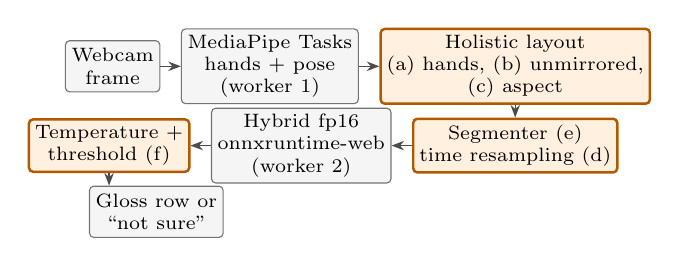
\begin{tikzpicture}[
  node distance=1.6mm and 2.6mm,
  box/.style={draw=black!55, rounded corners=1.5pt, fill=black!4, align=center, font=\scriptsize,
              inner sep=2.2pt, minimum height=6.5mm},
  live/.style={box, fill=orange!12, draw=orange!70!black, line width=0.9pt},
  arr/.style={-{Stealth[length=1.6mm]}, black!70, line width=0.45pt}]
  \node[box] (cam) {Webcam\\frame};
  \node[box, right=of cam] (mp) {MediaPipe Tasks\\hands + pose\\(worker 1)};
  \node[live, right=of mp] (map) {Holistic layout\\(a) hands, (b) unmirrored,\\(c) aspect};
  \node[live, below=of map] (seg) {Segmenter (e)\\time resampling (d)};
  \node[box, left=of seg] (cls) {Hybrid fp16\\onnxruntime-web\\(worker 2)};
  \node[live, left=of cls] (dec) {Temperature +\\threshold (f)};
  \node[box, below=of dec, xshift=6mm] (out) {Gloss row or\\``not sure''};
  \draw[arr] (cam) -- (mp);
  \draw[arr] (mp) -- (map);
  \draw[arr] (map) -- (seg);
  \draw[arr] (seg) -- (cls);
  \draw[arr] (cls) -- (dec);
  \draw[arr] (dec.south) -- (dec.south |- out.north);
\end{tikzpicture}
\caption{The live pipeline in the browser. The orange boxes with thick borders, marked (a)--(f),
are the six audited steps; \emph{Holistic layout} is the landmark layout of the training tracker.
Each step reads its constants from \cfg{features\_spec.json} or the model metadata, which the
Python training code also reads.}
\label{fig:pipeline}
\end{figure}
\fi

\subsection{Six candidate discrepancies}
\label{sec:faults}

\emph{(a) Hand slots.} Holistic, which produced the training data, crops each hand from the
pose, so its left-hand block is the hand at the signer's left wrist. The browser's
HandLandmarker reports a handedness label instead, and the shipped build mapped that label as if
the frame were mirrored while it ran detection on the unmirrored frame, so every hand went into the
wrong block. The fix assigns each detected hand to the block of the nearer pose wrist, Holistic's
own rule, and falls back to the label only when there is no pose.
\emph{(b) Mirroring.} The shipped build already detected on the unmirrored frame. Detection on
the mirrored frame, as a selfie pipeline would run it, is a counterfactual.
\emph{(c) Aspect ratio.} Normalized coordinates give a body different proportions in a portrait
phone recording and a wide webcam. The shipped build corrected this with a body-ratio estimate
over the first two seconds; the fix estimates the training data's width-to-height ratio
$r_{\mathrm{train}}$ from face geometry (\V{asp.train}) and rescales live y about the shoulder
midpoint by $k = r_{\mathrm{train}} / (w/h)$, with the frame's real width and height.
\emph{(d) Frame rate.} Training resampled by frame index (the dataset has no timestamps); the
browser's frame rate varies, so the fix resamples on the capture-time clock.
\emph{(e) Segmentation.} The shipped build segmented by hand presence: a segment starts after
\V{pres.start} frames with a hand and ends after \V{pres.end} without one or after \V{pres.max} s.
The fix is a state machine on motion energy, the speed of the wrist and fingertips on
aspect-corrected coordinates, with thresholds from the validation sequences.
\emph{(f) Calibration and abstention.} The shipped build showed the raw top-1 above a threshold
set for \V{cal.targetprec}\% precision on validation. The fix divides the logits by the validation
temperature and shows a word only above a validation threshold that maximizes the net score, in
which a correct accepted word gains one, a wrong one costs one and ``not sure'' scores zero.

Every constant above lives in \cfg{features\_spec.json}, which Python and the browser both read.
A golden-fixture test in continuous integration runs the browser code on the raw landmarks of
\V{par.cases} validation sequences exported from Python and requires every model input to match
within \V{par.tol} and the top-1 class to agree. It also covers hand assignment and replays a
stream through the segmenter.

\subsection{Evaluation on new recordings}

The author recorded \V{lg.clips} clips with a laptop webcam: \V{lg.signs} everyday signs from the
vocabulary, learned from online ASL video dictionaries, two takes each (median
\V{lg.duration}\,s), unmirrored at \V{lg.width}$\times$\V{lg.height} and about \V{lg.fps} frames
per second. The author is both the developer and the only signer, and a pilot with the same person
motivated the order of the fixes. No threshold or constant was fitted on these clips: every
threshold and constant comes from the training and validation splits, and the analysis was fixed
in the configuration before the first run (the repository cannot show this, as configuration and
results were committed together).

\emph{Python + Holistic} runs legacy MediaPipe Holistic, the tracker that produced the training
data, on every frame and then the Python live pipeline; it is deterministic. \emph{Browser +
Tasks} runs the web app in Chrome on the target laptop with the clip as a fake camera, in real
time, so frames drop as they would live. One browser per clip runs every configuration in a
seeded random order, three times each, and a clip's score is its mean over runs, so a browser clip
can change by a third. The baselines are the \emph{shipped build} itself (inference on the page's
main thread, \V{lg.web.c0headbuild.fps} frames per second) and \emph{as shipped}, the current app
with the shipped build's settings. A clip's prediction is the mean probability vector of its
classified segments; a clip without one counts as wrong, and the abstention threshold does not
enter clip scores. We report clip top-1 and top-3 with 95\% percentile bootstrap intervals over
clips \cite{efron1994bootstrap} and compare each configuration with the one it modifies by a
paired sign-flip test on per-clip scores \cite{dror2018hitchhiker}, Holm-corrected within each
pipeline and metric \cite{dror2017replicability} (\V{mde.py.family} top-1 comparisons in Python,
\V{mde.web.family} in the browser). This clip-level analysis was specified before the runs.
Because a sign's two takes are not independent, a sensitivity analysis added afterwards treats
each sign as one unit. Power is low: significance at the first Holm step needs at least
\V{mde.web.k} clips moving in one direction in the browser (\V{mde.web.pts} points if each moves
by a whole clip) and \V{mde.py.k} in Python, so smaller effects are inconclusive rather than
absent \cite{card2020power}.

\subsection{Results}
\label{sec:liveresults}

% Generated by scripts/paper_tables.py -- do not edit.
\typeout{[table livegap]}
\begin{table}[t]
\caption{Live-gap ablation}
\label{tab:livegap}
\centering
\footnotesize
\setlength{\tabcolsep}{3pt}
\begin{tabular}{lrrrr}
\toprule
 & \multicolumn{2}{c}{Python} & \multicolumn{2}{c}{Browser} \\
\cmidrule(lr){2-3}\cmidrule(lr){4-5}
Config & top-1 & top-3 & top-1 & top-3 \\
\midrule
Shipped build & -- & -- & \V{lg.web.c0headbuild.top1} & \V{lg.web.c0headbuild.top3} \\
As shipped (v1 CNN) & \V{lg.py.c0asshipped.top1} & \V{lg.py.c0asshipped.top3} & \V{lg.web.c0asshipped.top1} & \V{lg.web.c0asshipped.top3} \\
+ v2 hybrid model & \V{lg.py.c1model.top1} & \V{lg.py.c1model.top3}$^{*}$ & \V{lg.web.c1model.top1}$^{*}$ & \V{lg.web.c1model.top3}$^{*}$ \\
+ hand assignment (a) & \V{lg.py.c2hands.top1}$^{*}$ & \V{lg.py.c2hands.top3}$^{*}$ & \V{lg.web.c2hands.top1}$^{*}$ & \V{lg.web.c2hands.top3}$^{*}$ \\
+ aspect from frame (c) & \V{lg.py.c3aspect.top1} & \V{lg.py.c3aspect.top3} & \V{lg.web.c3aspect.top1} & \V{lg.web.c3aspect.top3} \\
+ time resampling (d) & \V{lg.py.c4time.top1} & \V{lg.py.c4time.top3} & \V{lg.web.c4time.top1} & \V{lg.web.c4time.top3} \\
+ motion segmenter (e) & \V{lg.py.c5segmenter.top1} & \V{lg.py.c5segmenter.top3} & \V{lg.web.c5segmenter.top1} & \V{lg.web.c5segmenter.top3} \\
+ calibration (f): final & \V{lg.py.c6final.top1} & \V{lg.py.c6final.top3} & \V{lg.web.c6final.top1} & \V{lg.web.c6final.top3} \\
\midrule
final, old hand mapping & \V{lg.py.xhands.top1}$^{*}$ & \V{lg.py.xhands.top3}$^{*}$ & \V{lg.web.xhands.top1}$^{*}$ & \V{lg.web.xhands.top3}$^{*}$ \\
final, mirrored frame (b) & -- & -- & \V{lg.web.xmirrored.top1} & \V{lg.web.xmirrored.top3} \\
final, mirrored + old mapping & -- & -- & \V{lg.web.xmirroredlabel.top1} & \V{lg.web.xmirroredlabel.top3} \\
final, no aspect corr. & \V{lg.py.xaspectoff.top1} & \V{lg.py.xaspectoff.top3} & \V{lg.web.xaspectoff.top1} & \V{lg.web.xaspectoff.top3}$^{*}$ \\
final, body-ratio aspect & \V{lg.py.xaspectcalibrated.top1} & \V{lg.py.xaspectcalibrated.top3} & \V{lg.web.xaspectcalibrated.top1} & \V{lg.web.xaspectcalibrated.top3} \\
final, index resampling & \V{lg.py.xindex.top1} & \V{lg.py.xindex.top3} & \V{lg.web.xindex.top1} & \V{lg.web.xindex.top3} \\
final, presence segmenter & \V{lg.py.xpresence.top1} & \V{lg.py.xpresence.top3} & \V{lg.web.xpresence.top1} & \V{lg.web.xpresence.top3} \\
final, v1 CNN & \V{lg.py.xv1model.top1} & \V{lg.py.xv1model.top3} & \V{lg.web.xv1model.top1} & \V{lg.web.xv1model.top3} \\
\bottomrule
\end{tabular}
\par\smallskip
\begin{minipage}{\linewidth}\footnotesize Live-gap ablation on the \V{lg.clips} webcam clips (\V{lg.signs} signs $\times$ 2 takes): clip-level top-1/top-3 (\%) for Python with MediaPipe Holistic and for the browser with MediaPipe Tasks. Upper block: one fix added per row; lower block: one fix of the final pipeline undone. Browser rows are means over three real-time runs; a dash marks a configuration that exists only in the browser. Clip scores do not use the abstention threshold. $^{*}$: the change against the row it modifies is significant after Holm correction within the pipeline and metric (clip as unit, as pre-specified). Top-1 intervals, raw and sign-level p-values are in the extended version~\cite{shukla2026manuvox}.\end{minipage}
\end{table}


Table~\ref{tab:livegap} gives the ablation. The shipped build recognized
\V{lg.web.c0headbuild.top1}\% of the clips (top-3 \V{lg.web.c0headbuild.top3}\%). With the hybrid
and all fixes, clip top-1 reaches \V{lg.web.c6final.top1}\% \V{lg.web.c6final.top1ci} in the
browser and \V{lg.py.c6final.top1}\% \V{lg.py.c6final.top1ci} in Python. Measured from the hybrid
with no fix, this recovers \V{lg.web.recover}\% (browser) and \V{lg.py.recover}\% (Python) of the
drop from its \V{m.d.top1}\% test top-1, so most of the gap remains. The test split excludes
sequences with too few hand frames while a clip without a segment counts as wrong, so this drop
somewhat overstates the live gap.

\paragraph*{Hand slots had by far the largest effect}
Adding the hand fix raised clip top-1 by \V{lg.py.c2hands.dtop1} points in Python and
\V{lg.web.c2hands.dtop1} in the browser (\V{lg.web.c2hands.dtop1better} clips better,
\V{lg.web.c2hands.dtop1worse} worse), and undoing it in the final pipeline cost
\V{lg.py.xhands.dtop1} and \V{lg.web.xhands.dtop1} points. In the pre-specified clip-level analysis
all four changes are significant after correction. With signs as the unit, they remain significant
in Python (Holm $p$ = \V{lg.py.c2hands.dtop1psign} and \V{lg.py.xhands.dtop1psign}) and for undoing
the fix in the browser (\V{lg.web.xhands.dtop1psign}), but not for adding it in the browser
(\V{lg.web.c2hands.dtop1psign}). Mirroring (b) was not shown to be a fault: once hands are
assigned by the pose, detecting on the mirrored frame changes clip top-1 by
\V{lg.web.xmirrored.dtop1} points \V{lg.web.xmirrored.dtop1ci}, compatible with no effect, and the
old label mapping fails with or without mirroring (\V{lg.web.xhands.top1}\% and
\V{lg.web.xmirroredlabel.top1}\%).

\paragraph*{Aspect correction and segmentation (inconclusive)}
Removing all aspect correction from the final pipeline cost \V{lg.py.xaspectoff.dtop1} points in
Python and \V{lg.web.xaspectoff.dtop1} in the browser, and in the cumulative ablation replacing
presence segmentation by the motion segmenter cost \V{lg.py.c5segmenter.dtop1} and
\V{lg.web.c5segmenter.dtop1}. None of these top-1 changes is significant after correction at
either unit. The final pipeline with presence segmentation matches or beats every other
configuration, \V{lg.py.xpresence.top1}\% in Python and \V{lg.web.xpresence.top1}\% in the browser.
The motion segmenter loses mostly whole signs it never segmented (\V{lg.py.c6final.noseg} clips in
Python and \V{lg.web.c6final.noseg} per browser run without a classified segment, against
\V{lg.py.xpresence.noseg} and \V{lg.web.xpresence.noseg}). Its thresholds assume the dataset's
frames are \V{seg.assumedfps} fps apart; if they are not, speeds are misestimated, which would
produce missed starts of this kind. We keep the pipeline as specified, because choosing a
segmenter on these clips would tune on the test.

\ifwithdetails
\paragraph*{The other changes}
Swapping in the hybrid before any fix gained \V{lg.web.c1model.dtop1} points in the browser and
\V{lg.py.c1model.dtop1} in Python, from a floor near zero. Resampling by time (d), which cannot
matter in Python, changed browser clip top-1 by \V{lg.web.c4time.dtop1} points, and calibration
(f) by \V{lg.web.c6final.dtop1}. Replacing the hybrid by the v1 CNN in the final pipeline cost
\V{lg.py.xv1model.dtop1} and \V{lg.web.xv1model.dtop1} points (\V{lg.web.xv1model.dtop1sig}), so
the hybrid's test-set advantage shows only weakly here.
\fi

\paragraph*{What remains}
Browser minus Python is \V{lg.pd.c6final.diff} points \V{lg.pd.c6final.ci} for the final pipeline
(signs as the unit). We see no evidence that the training tracker does better on these clips, but
the interval allows a sizeable advantage for Holistic, and the pipelines also differ in real-time
frame dropping. The rest of the gap lies in what both pipelines share, above all segmentation, or
in the clips themselves (signer, camera, room and the signer's productions), which this design
cannot separate. In both pipelines, \V{lg.failboth} of the \V{lg.signs} signs fail in every take.
Live, the calibration does not hold: the expected calibration error is \V{lg.cal.web.ece} in the
browser (\V{cal.test.ece1} on test), and the threshold accepts \V{lg.cal.web.cov}\% of segments at
\V{lg.cal.web.sel}\% selective accuracy.

\paragraph*{Training on webcam data (v3)}
Through the final pipeline, v3 reached clip top-1 \V{v3c.web.b}\% \V{v3c.web.bci} in the browser
and \V{v3c.py.b}\% \V{v3c.py.bci} in Python, against \V{v3c.web.a}\% and \V{v3c.py.a}\% for v2 in
the same runs: \V{v3c.web.diff} points in the browser (Holm $p$ = \V{v3c.web.p},
\V{v3c.web.sig}) and \V{v3c.py.diff} in Python ($p$ = \V{v3c.py.p}, \V{v3c.py.sig}). Both
differences favor v3, but neither is significant with fifty clips: v3's added data and
augmentation narrowed this signer's gap far less than they raised its in-domain ASL Citizen score,
if at all. v3 recognizes \V{cit.v3.top1}\% of the videos of ASL Citizen's unseen signers, trimmed
to the sign, but under half of these clips. That is consistent with segmentation or this signer's
productions, more than webcam conditions as such, limiting the live score, but an in-domain score
cannot settle it.

\subsection{Personalization (Teach Dex)}
\label{sec:teach}

For each sign a user has taught, Teach Dex takes the highest cosine similarity $s_c$ between a
segment's embedding (the model's \V{td.embdim}-value penultimate layer) and the user's examples
of sign $c$, and adds $w\,(s_c - b)$ to that sign's calibrated logit; the weight $w$
(\V{td.v2.weight}) and offset $b$ (\V{td.v2.offset}) were fitted on validation signers, not on
the user's clips. In a separate record-then-test evaluation, take 1 of each sign supplied up to
\V{td.examples} examples, all from one production, and take 2 was recognized with them in
\V{td.v2.runs} browser runs. With v2, clip top-1 on take 2
rose from \V{td.v2.model}\% \V{td.v2.modelci} to \V{td.v2.teach}\% \V{td.v2.teachci},
\V{td.v2.diff} points \V{td.v2.ci} (Holm $p$ = \V{td.v2.p}, \V{td.v2.sig}). In a control that
taught only \V{td.v2.half} of the signs, the untaught signs changed by \V{td.v2.harm} points. This
is the feature's best case: one signer, both takes recorded in one sitting, and the test
vocabulary equal to the signs offered for teaching. A v3 run of the same test was compromised by
its harness; the extended version reports it.

\section{Limitations and Ethical Considerations}
\label{sec:limitations}

The live evaluation uses \V{lg.clips} clips recorded by a single signer, the author, in one room
with one laptop camera. The author is not a fluent signer; the signs in the live recordings were
learned from online ASL video dictionaries, and how the \V{lg.signs} signs were chosen was not
recorded. If the signer's productions differ from the dataset's signers, some live errors are
production differences rather than pipeline or camera effects, and nothing in this design
separates them. The results show which pipeline discrepancies matter for this signer and camera;
they do not estimate accuracy for Deaf signers in general. Two controls would locate the remaining
gap: running the live pipeline on test-split landmark sequences, and an oracle segmentation of the
live clips. The ASL Citizen label mapping is AI-assisted and unconfirmed by a signer, and v3's
in-domain accuracy does not validate it. The live clips are not an independent test of v3 either:
they were analyzed before v3's webcam augmentation was designed. The model recognizes
\V{data.signs} isolated signs; it does not handle continuous signing, fingerspelling, or signs
outside the vocabulary, and it is not a translator. The author is based in India, where Indian
Sign Language is the relevant language; nothing here transfers to it without new data.

We did not evaluate the system with Deaf or hard-of-hearing users, and no Deaf signer took part in
its design. Sign language technology should be built with, and ideally led by, Deaf communities
\cite{bragg2019interdisciplinary,yin2021including,fox2023bestpractices}, and Deaf researchers have
criticized how often the field sets its agenda without them \cite{desai2024systemic}. At the live
accuracy we measured, the app's Practice mode, which scores a sign against a target, would tell a
learner that many correctly produced signs are wrong; it should be evaluated with learners and
Deaf teachers before anyone relies on it. The live clips show the author, who consents to their use here; they are not
released, and no ASL Citizen data or model trained on it is released either. When the user asks
the app for a sentence, only the recognized glosses are sent to a third-party language model
provider. The code, configurations and result files behind every number are in the repository of
the extended version \cite{shukla2026manuvox}.

\section{Conclusion}
\label{sec:conclusion}

A signer-independent test accuracy of \V{m.d.top1}\% did not make a usable live recognizer: the
first deployment recognized \V{lg.web.c0headbuild.top1}\% of new webcam clips. Of six candidate
train--serve discrepancies, one had a large and consistent effect: putting each hand in a different
slot from the one the training tracker used. A shared feature specification and a golden parity
test, which covers hand assignment, now keep the Python and browser pipelines identical and fail
when they diverge. With the fixes, clip top-1 reaches \V{lg.web.c6final.top1}\% in the browser and
\V{lg.py.c6final.top1}\% with the training tracker, about \V{lg.web.recover}--\V{lg.py.recover}\%
of the way back to test accuracy. The rest of the gap is shared by both live pipelines. Part of it
is a segmenter, tuned on dataset sequences, that missed whole signs; the rest may be the signer,
the camera or the signer's productions, which one signer cannot separate. Thresholds chosen on
dataset sequences need live validation data of their own, and the next steps are an oracle
segmentation of these clips and live recordings from many Deaf signers, gathered with their
involvement.

\section*{Acknowledgment}

Anthropic's Claude and Claude Code assisted me throughout this project: Claude Code helped
write the training, evaluation and browser inference code, and both tools helped draft and edit
the manuscript text and tables. I reviewed and checked all generated code and every reported
number myself, and I take full responsibility for the results presented here.


\bibliographystyle{IEEEtran}
\bibliography{ieee_control,../references}

\end{document}
